\chapter{Density functional theory as a screening method for dense metal membranes}

\section{Abstract}

\section{Introduction}
High impurity resistant dense metal membranes are being developed for hydrogen impurity enrichments of HRS samples with hydrogen derived from biomass, hydrocarbon or electrolysis. Metal membranes operate by selectively dissociating hydrogen, which then allows the hydrogen atoms to solubilize and subsequently permeate through the bulk of the separation layer. The problem is that many hydrogen impurities are also capable of adsorbing onto and interacting with the surface of many of the metals which comprise dense metal membranes. The impact of this adsorption can vary depending the molecule, Carbon monoxide for example will simply adsorb onto the surface and result in competitive adsorption between the hydrogen and impurity. Sulphur containing impurities which are commonly found in hydrocarbon sources and therefore are potentially present in any hydrogen produced from these methods. Sulphur containing impurities present more of a problem since they can potentially react with many metals used for hydrogen separation membranes. The impact of these contaminants can be minimized by designing alloy compositions that have a weaker attraction to the membrane, and therefore will have less of an affect at higher temperatures where these membranes operate.

Physically testing each potential membrane composition would be time consuming and costly due to the high price of palladium, the time required to synthesise specific membrane compositions, and performing the tests. Simulations provide a solution to this, allowing potential alloys to be screened for their interaction strength with each individual ISO 14687-2 impurity quickly, avoiding the cost of manufacturing each alliy composition. 

This chapter will calculate the behaviour of 14 palladium alloy composition under 13 ISO 14687-2 impurities. This is done by comparing the total energy of different configurations after relaxation of internal forces in the system. The close packed surfaces of palladium alloys were simulated as 

\section{Results and discussion}


\begin{table}[]
    \centering
    \caption{Simulated total energy values of ISO 14687-2 impurities}
    \label{gases}
    \begin{tabular}{@{}cc@{}}
    \toprule
    Gas          & \begin{tabular}[c]{@{}c@{}}Total Energy\\ $(kJ \times 10^{-21})$\end{tabular} \\ \midrule
    H            & -2.01                                                               \\
    N\textsubscript{2}           & -123.91                                                             \\
    O\textsubscript{2}           & -180.86                                                             \\
    CO           & -130.93                                                             \\
    CO\textsubscript{2}          & -221.95                                                             \\
    NH\textsubscript{3}          & -1933.22                                                            \\
    Ar           & -208.10                                                             \\
    CH\textsubscript{4}          & -50.73                                                              \\
    Formaldehyde & -136.13                                                             \\
    Formic Acid  & -227.08                                                             \\
    H\textsubscript{2}S          & -150.36                                                             \\
    He           & -12.62                                                              \\
    H\textsubscript{2}O          & -95.99                                                              \\ \bottomrule
    \end{tabular}
\end{table}

\subsection{Stability of palladium alloy compositions}
Hydrogen adsorption on the surface of palladium is a key value for the purpose of this experiment. The affinity for a palladium alloy to adsorb on the surface is the initial step for hydrogen permeation, and below a certain thickness becomes the rate limiting step. As expected all alloys had an affinity for hydrogen adsorption and these values matched what is generally found in literature. These values will be compared to the adsorption energies of other impurities on the alloys in order to determine their resistance to the impurity. The adsorption energies of hydrogen on a the Pd slab system is shown in figure \ref{Pdsite}. In a Pd system hydrogen preferentially adsorbs on the FCC and top sites at relativley even energies. At both of these sites hydrogen is able to form a stable system without being affected by other forces. HCP and top sites have a  lower affinity for hydrogen adsorption and this is likely due to the influence of competition by neighbouring sites which can provide higher stability.
Hydrogen adsorption on the surface of palladium is a key value for the purpose of this experiment. The affinity for a palladium alloy to adsorb on the surface is the initial step for hydrogen permeation, and below a certain thickness becomes the rate limiting step. As expected all alloys had an affinity for hydrogen adsorption and these values matched what is generally found in literature. These values will be compared to the adsorption energies of other impurities on the alloys in order to determine their resistance to the impurity. The adsorption energies of hydrogen on a the Pd slab system is shown in figure \ref{Pdsite}. In a Pd system hydrogen preferentially adsorbs on the FCC and top sites at relativley even energies. At both of these sites hydrogen is able to form a stable system without being affected by other forces. HCP and top sites have a  lower affinity for hydrogen adsorption and this is likely due to the influence of competition by neighbouring sites which can provide higher stability.
Hydrogen adsorption on the surface of palladium is a key value for the purpose of this experiment. The affinity for a palladium alloy to adsorb on the surface is the initial step for hydrogen permeation, and below a certain thickness becomes the rate limiting step. As expected all alloys had an affinity for hydrogen adsorption and these values matched what is generally found in literature. These values will be compared to the adsorption energies of other impurities on the alloys in order to determine their resistance to the impurity. The adsorption energies of hydrogen on a the Pd slab system is shown in figure \ref{Pdsite}. In a Pd system hydrogen preferentially adsorbs on the FCC and top sites at relativley even energies. At both of these sites hydrogen is able to form a stable system without being affected by other forces. HCP and top sites have a  lower affinity for hydrogen adsorption and this is likely due to the influence of competition by neighbouring sites which can provide higher stability.


\begin{table}[]
    \centering
    \caption{Simulated total energy values of alloy slabs}
    \label{slabs}
    \begin{tabular}{@{}cccc@{}}
    \toprule    
    Alloy/Metal Composition      & \begin{tabular}[c]{@{}c@{}}Total Energy\\ (ry)\end{tabular} & Total Energy (kJ) \\ \midrule
    Pd                       & -6653.38                                      & $-1.45\times10^{-17}$     \\
    PdAg\textsubscript{23}                   & -6774.37                                      & $-1.48\times10^{-17}$    \\
    PdAu\textsubscript{10}                   & -7545.53                                      & $-1.64\times10^{-17}$     \\
    PdAu\textsubscript{20}                   & -8437.613                                     & $-1.84\times10^{-17}$     \\
    Pd\textsubscript{60}Cu\textsubscript{40}                 & -5703.15                                      & $-1.24\times10^{-17}$     \\
    Pd\textsubscript{80}Cu\textsubscript{20}                 & -6178.29                                      & $-1.35\times10^{-17}$     \\
    Pd\textsubscript{70}Au\textsubscript{20}Zr\textsubscript{10}             & -8389.61                                      & $-1.83\times10^{-17}$     \\
    Pd\textsubscript{70}Cu\textsubscript{20}Zr\textsubscript{10}             & -6130.29                                      & $-1.34\times10^{-17}$     \\
    Pd\textsubscript{70}Ag\textsubscript{10}Zr\textsubscript{20}             & -6605.75                                      & $-1.44\times10^{-17}$     \\
    PdZr\textsubscript{10}                   & -6605.45                                      & $-1.44\times10^{-17}$     \\
    PdZr\textsubscript{20}                   & -6557.46                                      & $-1.43\times10^{-17}$     \\
    Pd\textsubscript{70}Au\textsubscript{20}Ag\textsubscript{10}             & -8485.99                                      & $-1.84\times10^{-17}$     \\
    Pd\textsubscript{70}Au\textsubscript{20}Cu\textsubscript{10}             & -8200.05                                      & $-1.79\times10^{-17}$     \\
    Pd\textsubscript{70}Cu\textsubscript{20}Ag\textsubscript{10}             & -6226.71                                      & $-1.36\times10^{-17}$     \\ \bottomrule
    \end{tabular}
    \end{table}
    Hydrogen adsorption on the surface of palladium is a key value for the purpose of this experiment. The affinity for a palladium alloy to adsorb on the surface is the initial step for hydrogen permeation, and below a certain thickness becomes the rate limiting step. As expected all alloys had an affinity for hydrogen adsorption and these values matched what is generally found in literature. These values will be compared to the adsorption energies of other impurities on the alloys in order to determine their resistance to the impurity. The adsorption energies of hydrogen on a the Pd slab system is shown in figure \ref{Pdsite}. In a Pd system hydrogen preferentially adsorbs on the FCC and top sites at relativley even energies. At both of these sites hydrogen is able to form a stable system without being affected by other forces. HCP and top sites have a  lower affinity for hydrogen adsorption and this is likely due to the influence of competition by neighbouring sites which can provide higher stability.
    Hydrogen adsorption on the surface of palladium is a key value for the purpose of this experiment. The affinity for a palladium alloy to adsorb on the surface is the initial step for hydrogen permeation, and below a certain thickness becomes the rate limiting step. As expected all alloys had an affinity for hydrogen adsorption and these values matched what is generally found in literature. These values will be compared to the adsorption energies of other impurities on the alloys in order to determine their resistance to the impurity. The adsorption energies of hydrogen on a the Pd slab system is shown in figure \ref{Pdsite}. In a Pd system hydrogen preferentially adsorbs on the FCC and top sites at relativley even energies. At both of these sites hydrogen is able to form a stable system without being affected by other forces. HCP and top sites have a  lower affinity for hydrogen adsorption and this is likely due to the influence of competition by neighbouring sites which can provide higher stability.
    Hydrogen adsorption on the surface of palladium is a key value for the purpose of this experiment. The affinity for a palladium alloy to adsorb on the surface is the initial step for hydrogen permeation, and below a certain thickness becomes the rate limiting step. As expected all alloys had an affinity for hydrogen adsorption and these values matched what is generally found in literature. These values will be compared to the adsorption energies of other impurities on the alloys in order to determine their resistance to the impurity. The adsorption energies of hydrogen on a the Pd slab system is shown in figure \ref{Pdsite}. In a Pd system hydrogen preferentially adsorbs on the FCC and top sites at relativley even energies. At both of these sites hydrogen is able to form a stable system without being affected by other forces. HCP and top sites have a  lower affinity for hydrogen adsorption and this is likely due to the influence of competition by neighbouring sites which can provide higher stability.


\subsection{Hydrogen and Impurity adsorption on palladium alloy membranes}\label{Hsection}
\subsubsection{Hydrogen}
Hydrogen adsorption on the surface of palladium is a key value for the purpose of this experiment. The affinity for a palladium alloy to adsorb on the surface is the initial step for hydrogen permeation, and below a certain thickness becomes the rate limiting step. As expected all alloys had an affinity for hydrogen adsorption and these values matched what is generally found in literature. These values will be compared to the adsorption energies of other impurities on the alloys in order to determine their resistance to the impurity. The adsorption energies of hydrogen on a the Pd slab system is shown in figure \ref{Pdsite}. In a Pd system hydrogen preferentially adsorbs on the FCC and top sites at relativley even energies. At both of these sites hydrogen is able to form a stable system without being affected by other forces. HCP and top sites have a  lower affinity for hydrogen adsorption and this is likely due to the influence of competition by neighbouring sites which can provide higher stability. The average adsorption energies of hydrogen on the surface of all palladium alloy slab systems are shown in figure \ref{h2ads}.

\begin{figure}
  \centering
  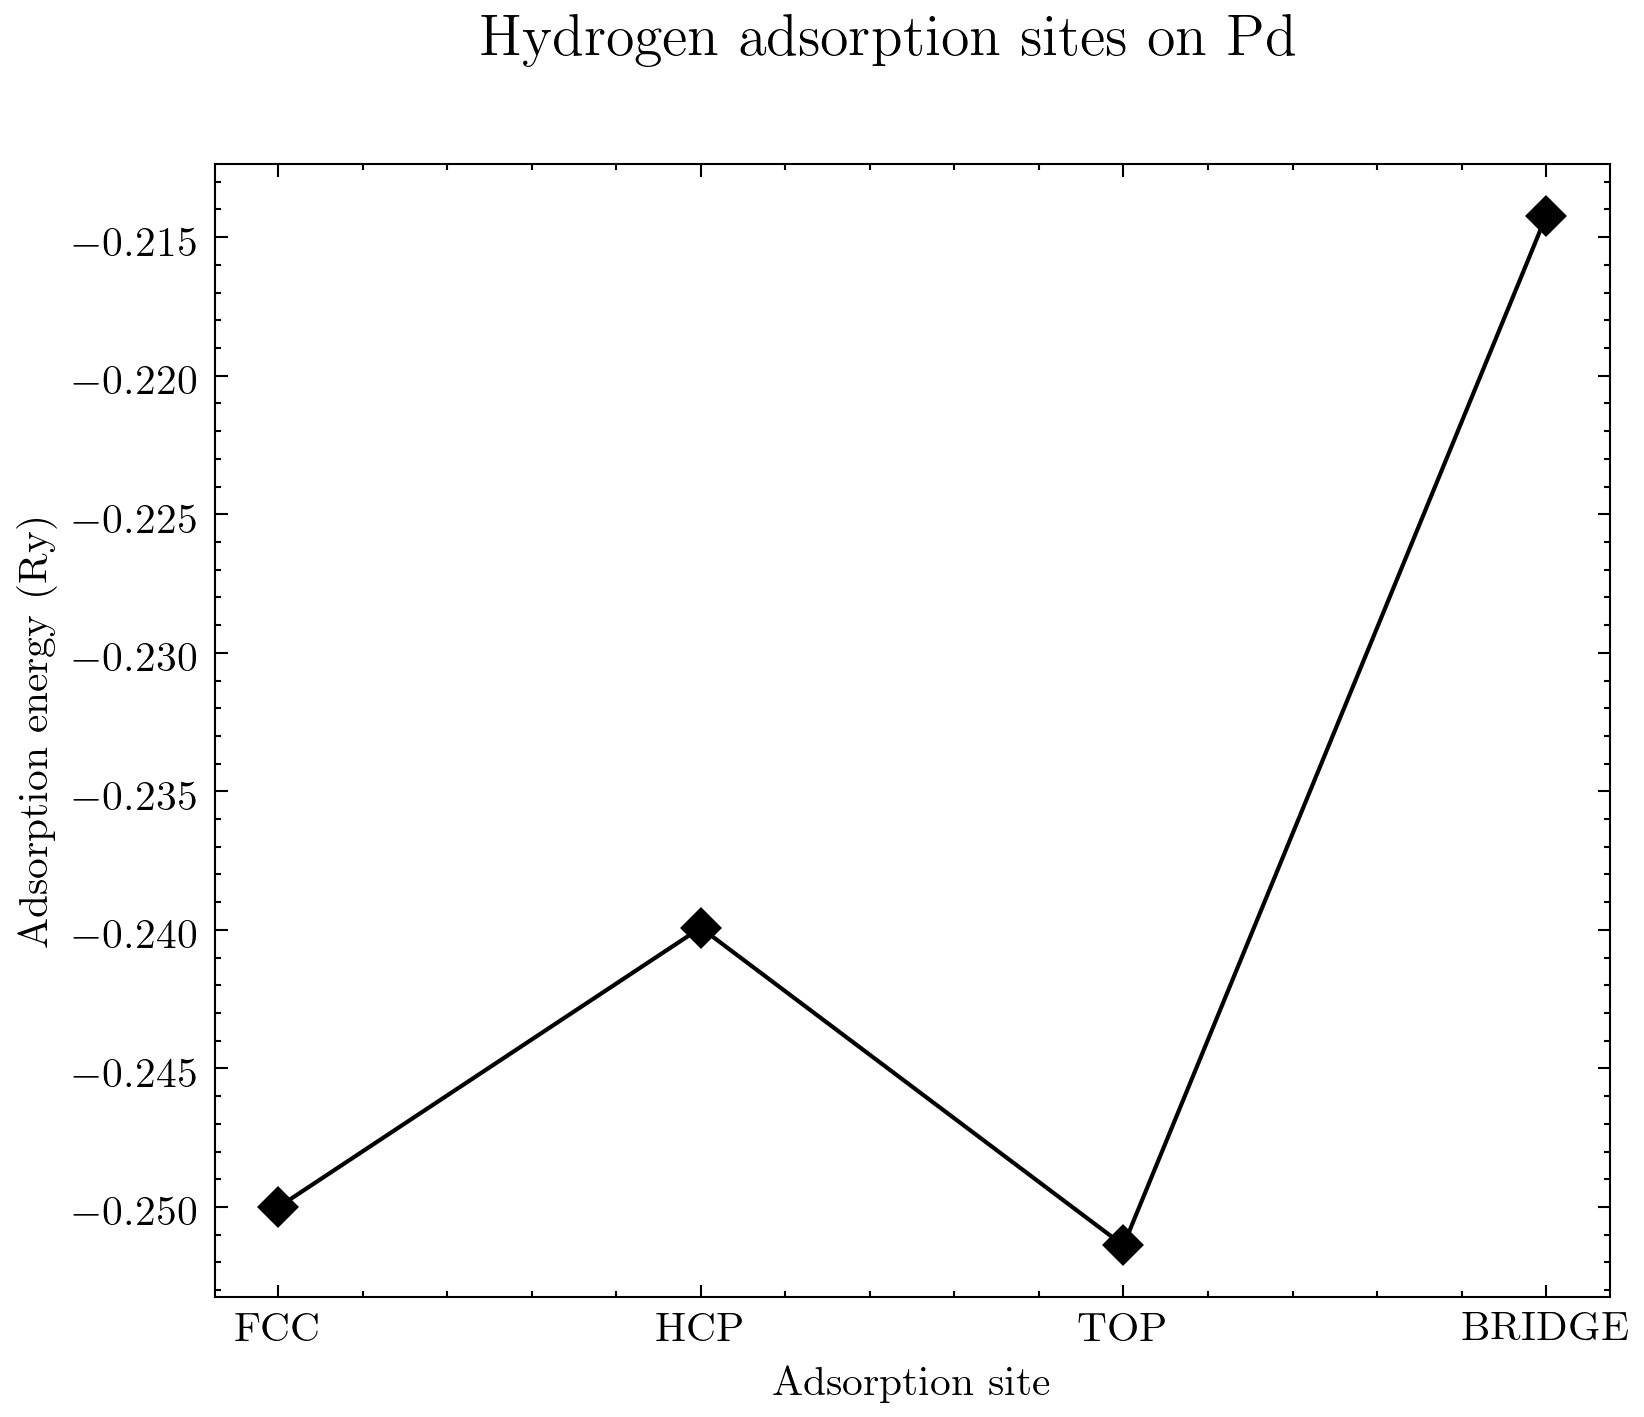
\includegraphics{/Users/marc/Thesis/Chapter3/data/PDSITES.jpg}
  \caption{Adsorption energy of H for each site on a 2x2x5 Pd slab}
  \label{Pdsite}
\end{figure}

Almost all binary alloys show a decreased affinity towards hydrogen adsoprtoion. This is due to hydrogen adsorption energies being closely related to the catalytic activity for hydrogen dissociation of the individual metal elements. The effect appears to be less prevalent for binary alloys with elements with a larger atomic size such as silver which is likely due to the larger atomic size creating a larger area for hydrogen to adsorb within fcc site of the crystalline lattice, which is one of the preferential sites for H adsorption. Zr and Au do not follow this trend however which indicates that the catalytic activity is effected more by electronic interactions than surface geometry. In all cases reduction in palladium from the surface results in lower catalytic activity for hydrogen adsorption which is also likely to be due to the average reduction in number of top sites avaliable for adsorption, which other than fcc is one of the preferential adsorption sites. 

All ternary alloys similarly showed lower catalytic activity than both Pd, and all binary alloys. This again shows that lowering the concentration of Pd in the surface of a membrane has the overall effect of lowering it's catalytic activity for hydrogen adsorption and dissociation with the exception of copper. The ternary alloys with the highest catalytic activity were PdAuAg and PdCuAg which previous experimental results showing that these alloys have higher permeability than other ternary alloys. All Zr containing alloys had lower catalytic activity showing that for hydrogen permeation Zr has the greatest inhibiting effect. The detrimental effects of Zr to the catalytic activity can be lessened by the addition of Au, Ag, or Cu however all are still lower than binary alloys. 

The correlation coefficient for the presence of each metal and it's effect on the resulting adsorption energy was calculated and is shown in table \ref{corrH}. It shows that the resulting inhibiting effect of each element follows the order Ag$<$Cu$<$Au$<$Zr. 

This value is an important benchmark for the following tests and will be compared to the resulting adsorption energies for other impurities. If these impurities show a lower adsorption energy value when compared to hydrogen then they will be preferntially adsorbed and less suitable for use for that type of impurity. It also reveals that the composition of the membrane can largely effect the catalytic activity for dissociation of hydrogen in itself. As membranes become thinner this will result in a shift of the limiting step to catalytic activity and therefore this value must also be optimised to ensure the highest flux can be achieved, however such work is outside the scope of this study. 

\begin{table}[]
  \centering
  \caption{Correlation coefficient of Ag, Au, Cu, Zr addition to Pd with adsorption energy of H}
  \label{corrH}
  \begin{tabular}{@{}cc@{}}
  \toprule
  Metal & Correlation coefficient \\ \midrule
  Ag    & -0.024666               \\
  Au    & 0.259205                \\
  Cu    & 0.019221                \\
  Zr    & 0.347930                \\ \bottomrule
  \end{tabular}
  \end{table}

\begin{landscape}
\begin{figure}
    \centering
    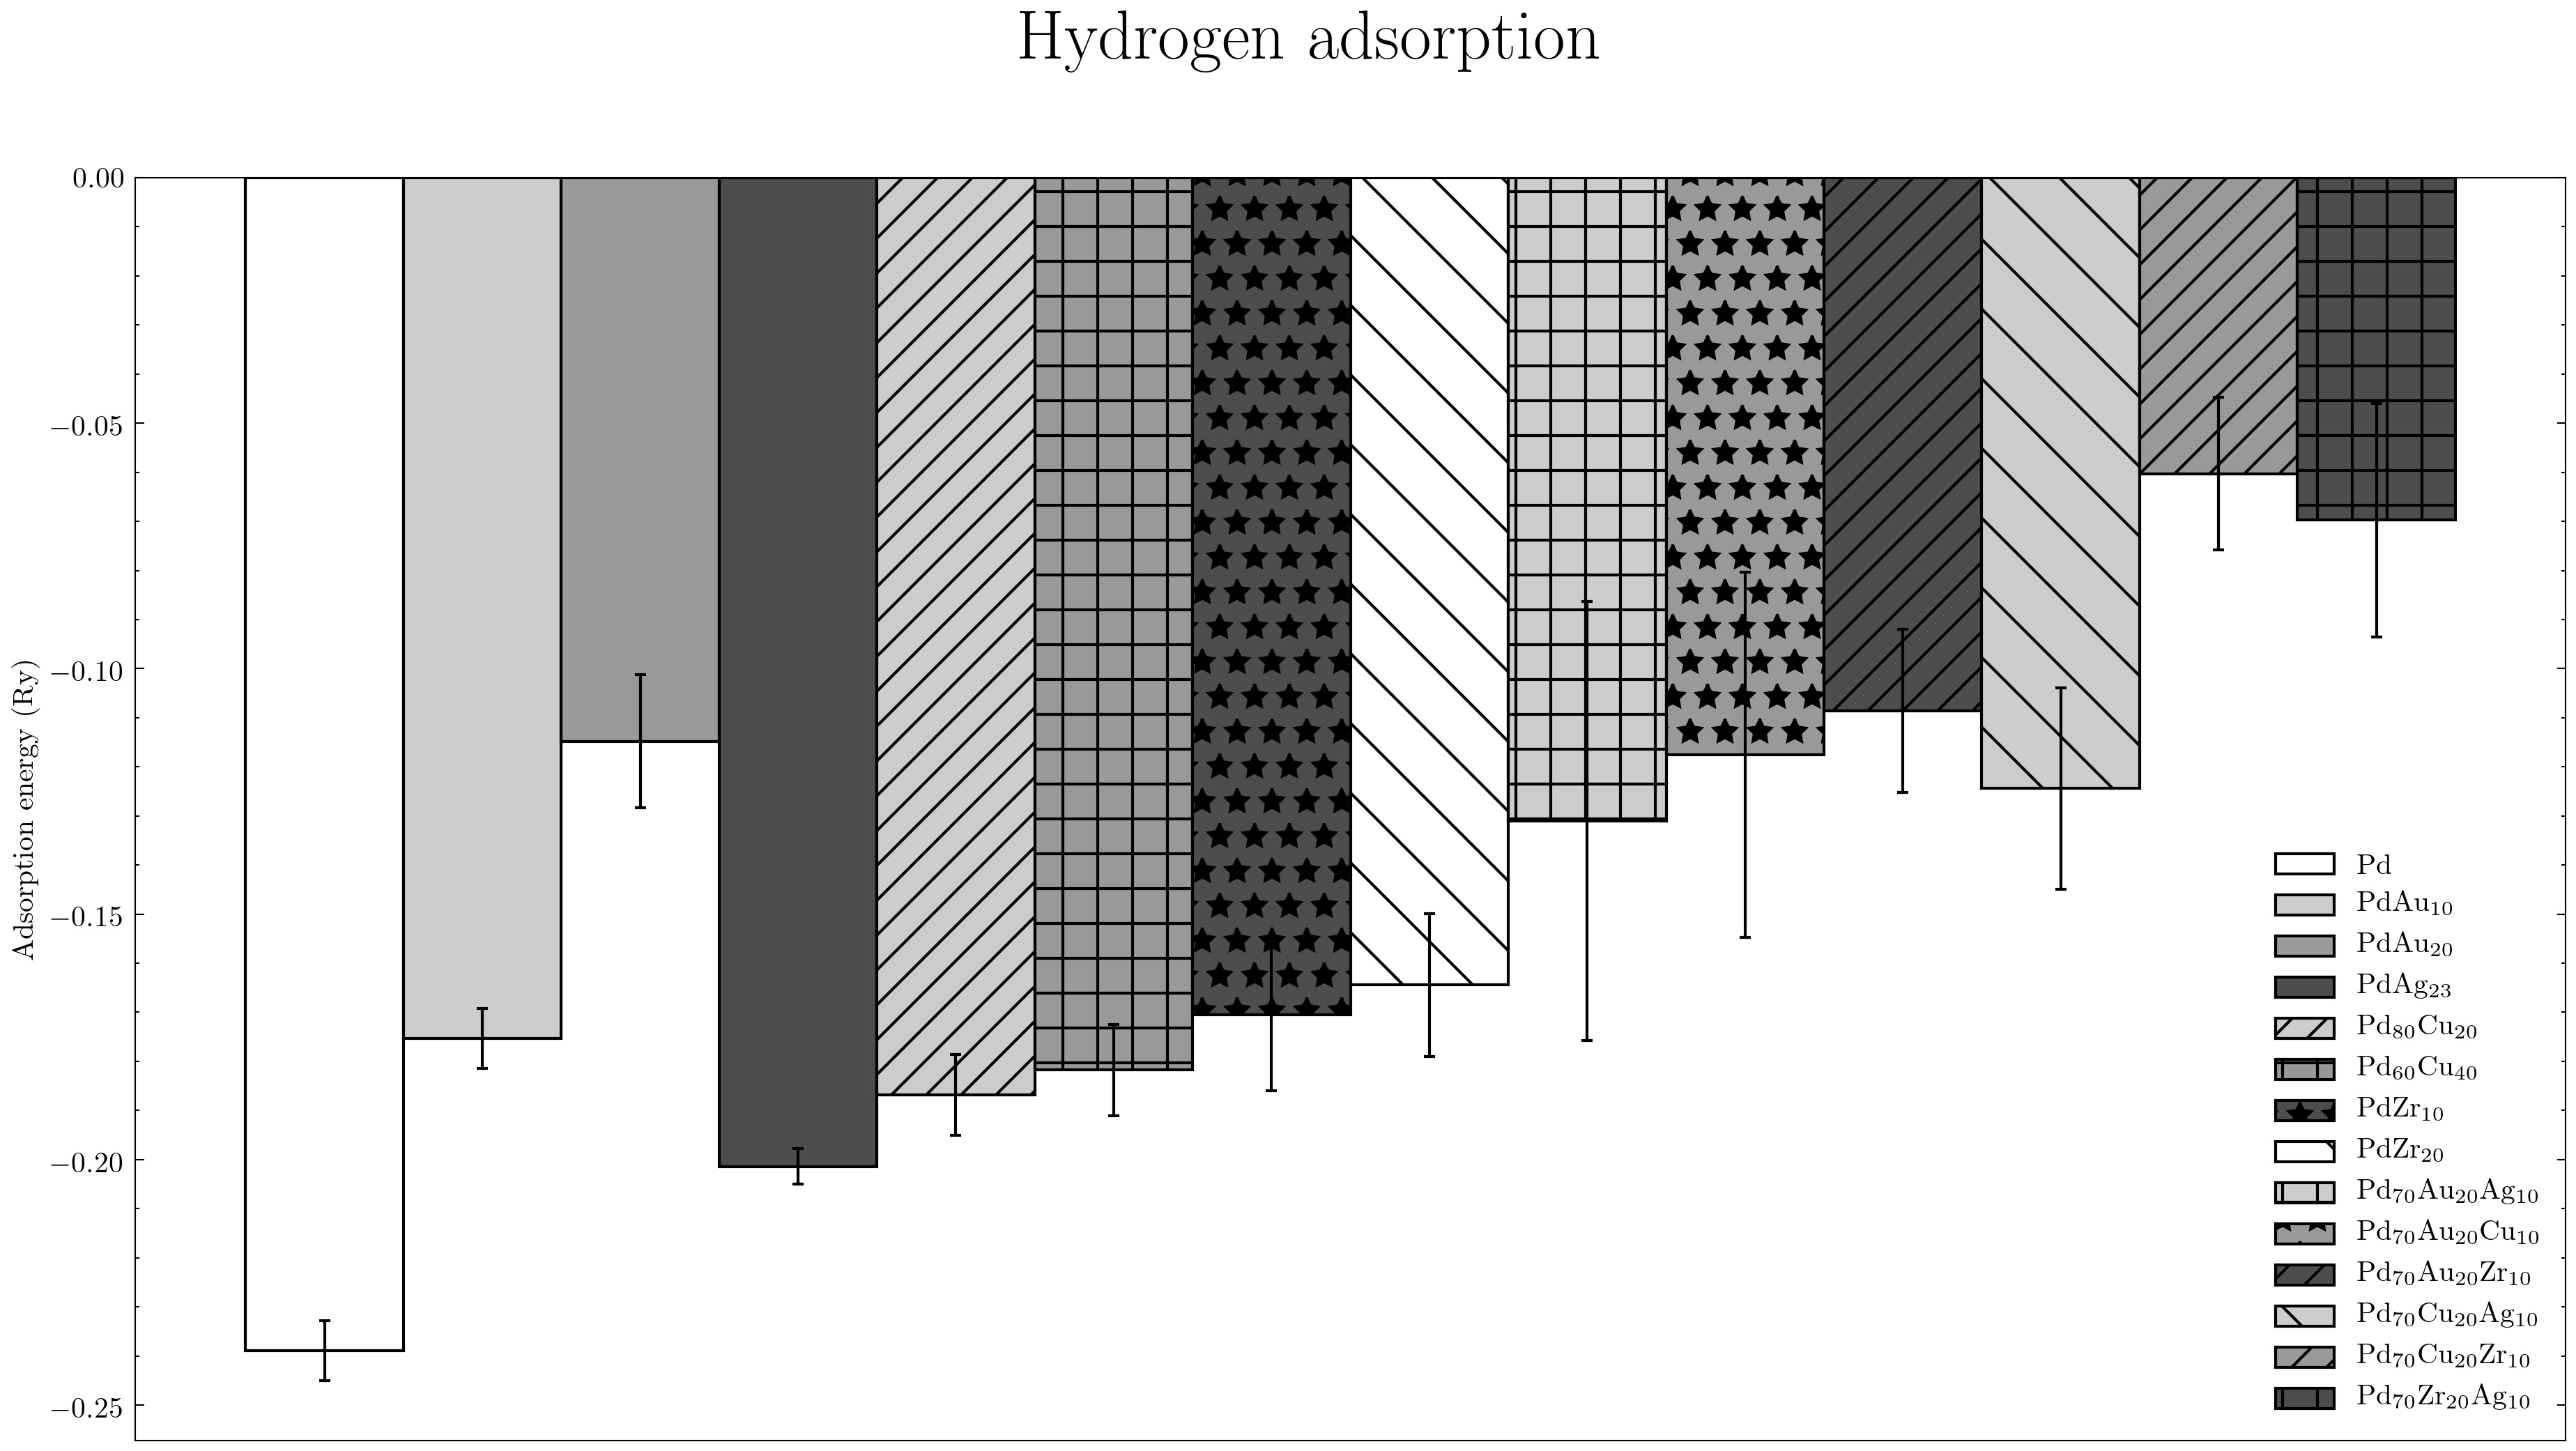
\includegraphics[width=0.9\linewidth,height=\textheight, keepaspectratio]{/Users/marc/Thesis/Chapter3/data/h2ads.jpg}
    \caption{Average adsorption energy of H\textsubscript{2} on the surface of palladium and palladium alloy slabs}
    \label{h2ads}
  \end{figure}

\end{landscape}
\subsubsection{Helium, Nitrogen, Carbon Dioxide and Argon}
Helium, Nitrogen, Argon, and CO\textsubscript{2} all represent the inert components in fuel cell hydrogen which do not effect the electrocatalyst and are therefore also likely to be inert to palladium membranes. The adsorption energies of these molecules on the surface of all the simulated palladium alloy slab systems are shown in figures \ref{heads} (He), \ref{n2ads} (N\textsubscript{2}), \ref{co2ads} (CO\textsubscript{2}) and \ref{Arads} (Ar). All these systems showed a positive adsorption energy meaning there will be no competitive adsorption taking place between these gases and hydrogen for the surface adsorption sites. These systems were also largely unstable as shown by the large errors associated with the results. Both of these facts suggest that none of these compounds will interfere with the operation of a palladium membrane.

\begin{figure}
  \centering
  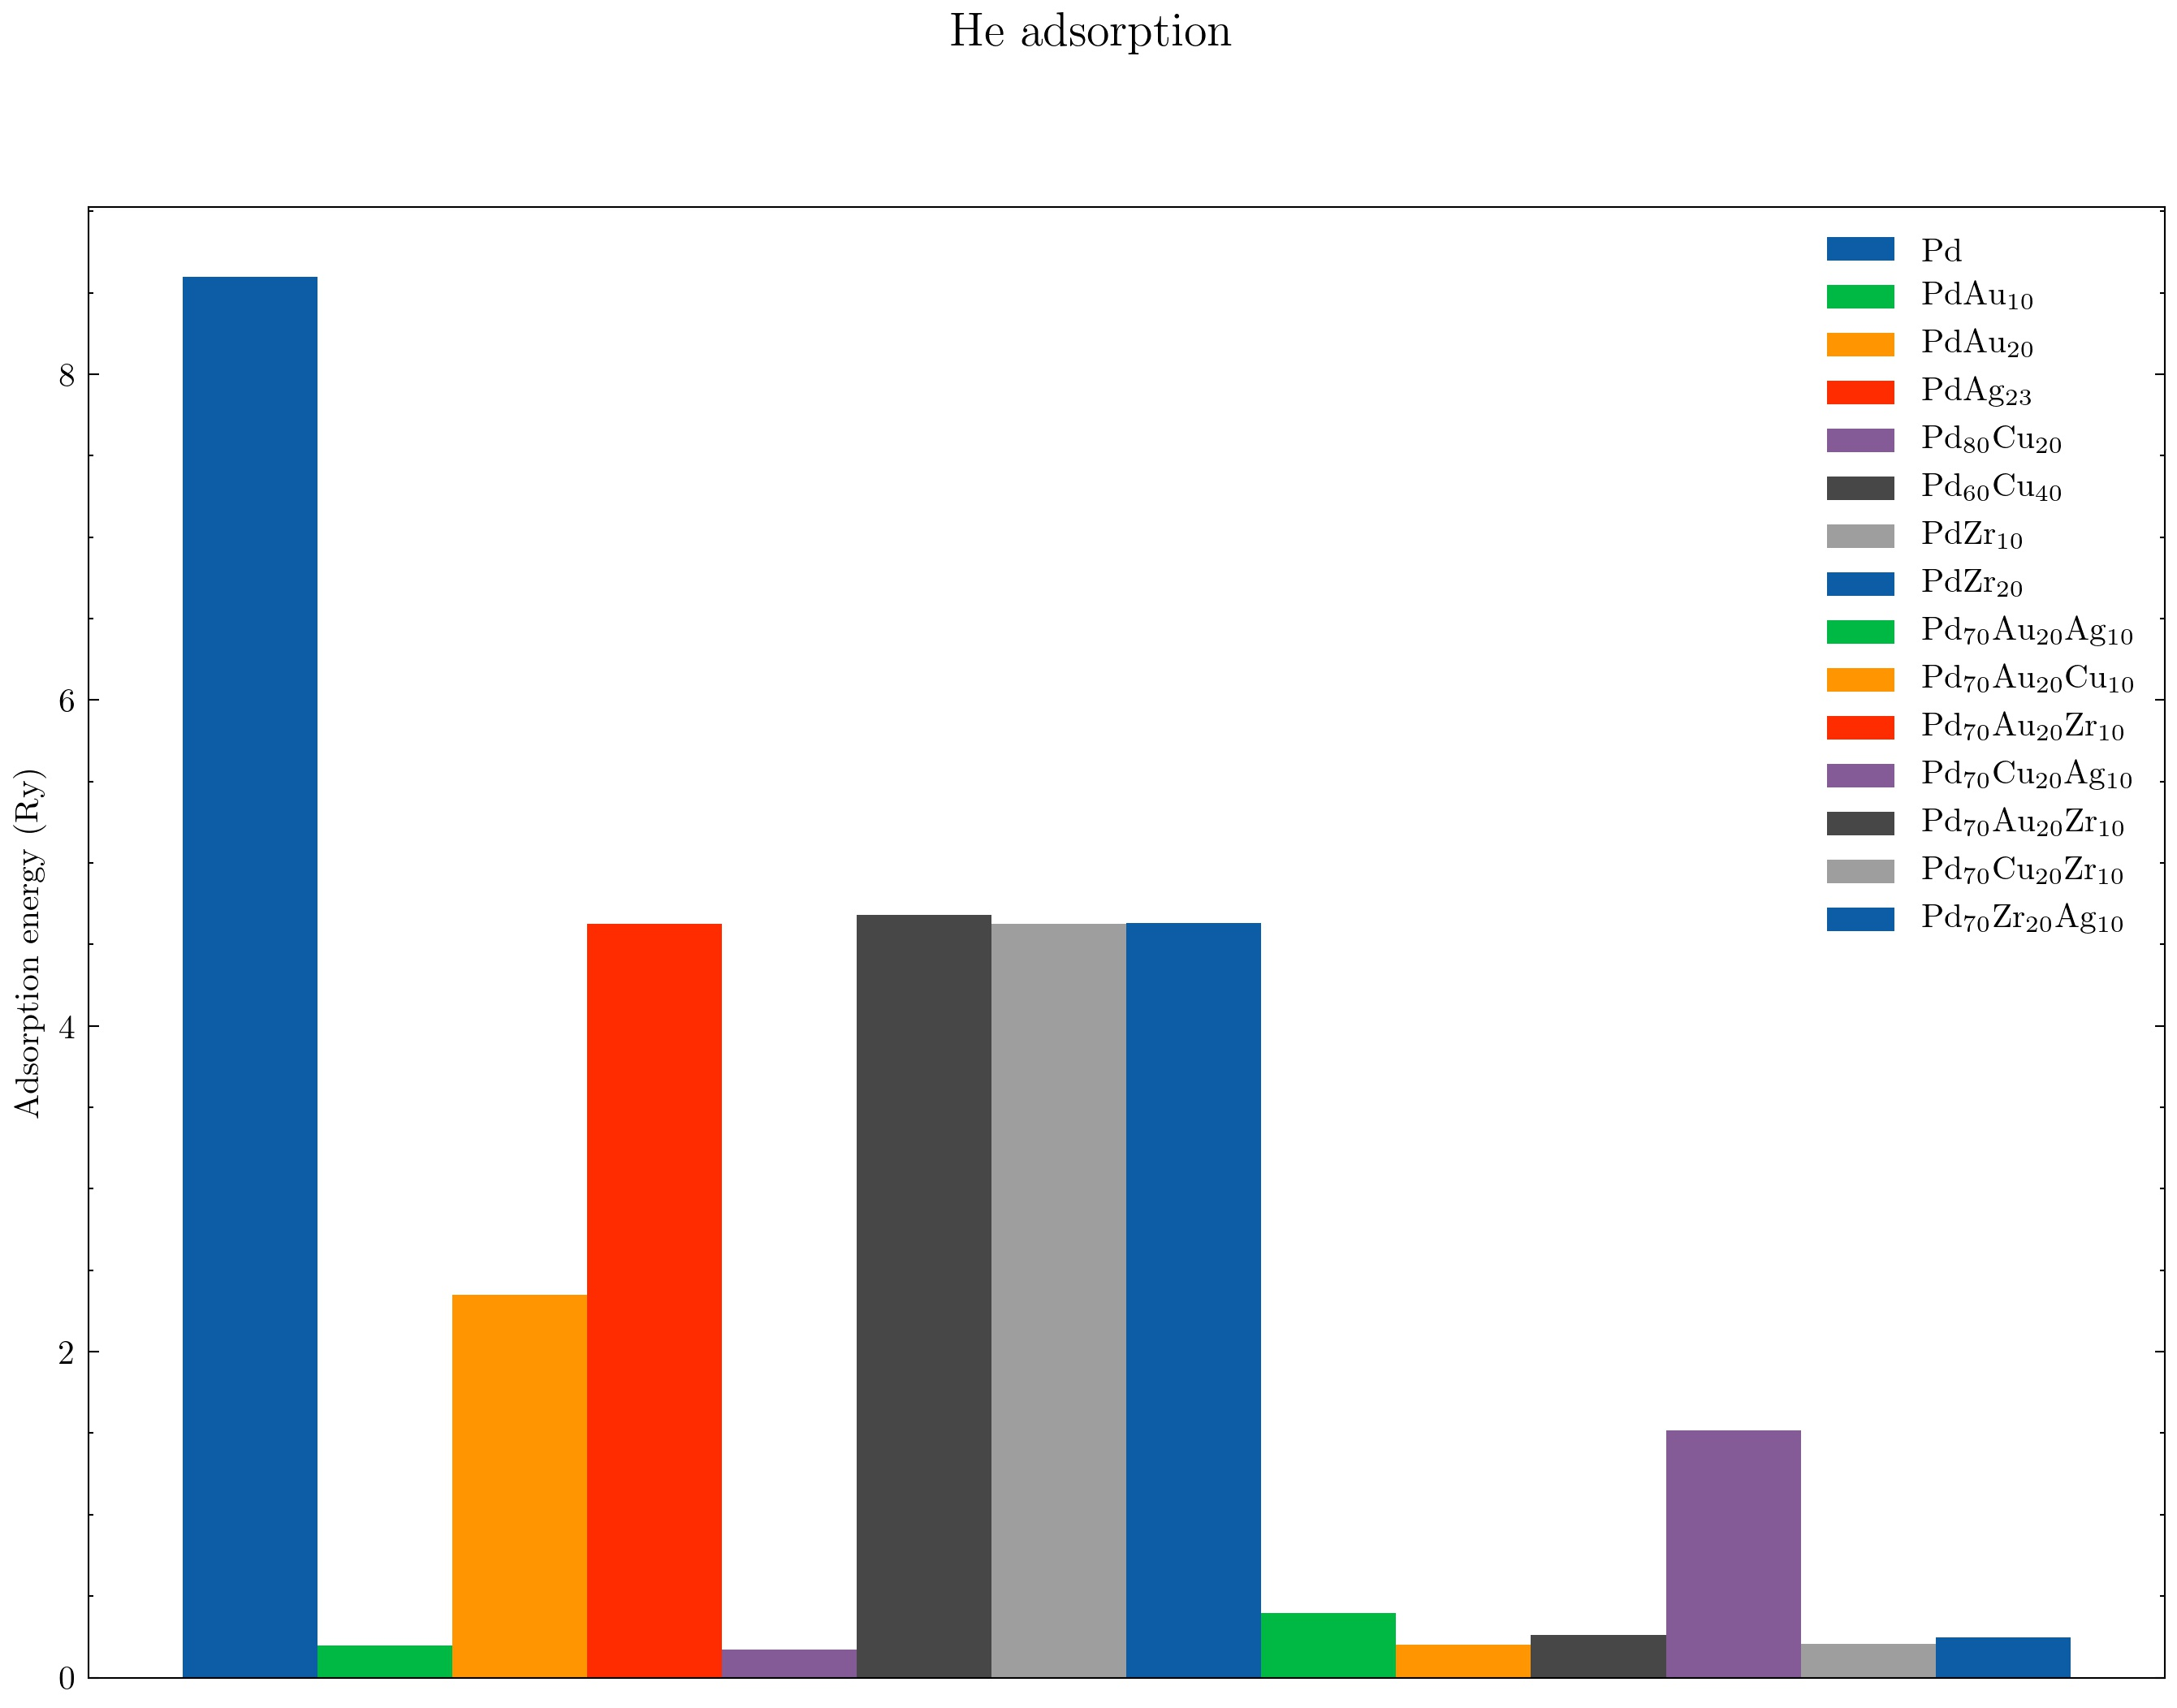
\includegraphics[width=0.9\linewidth, keepaspectratio]{/Users/marc/Thesis/Chapter3/data/HEads.jpg}
  \caption{Average adsorption energy of He on the surface of palladium and palladium alloy slabs}
  \label{heads}

\end{figure}

    \begin{figure}
        \centering
        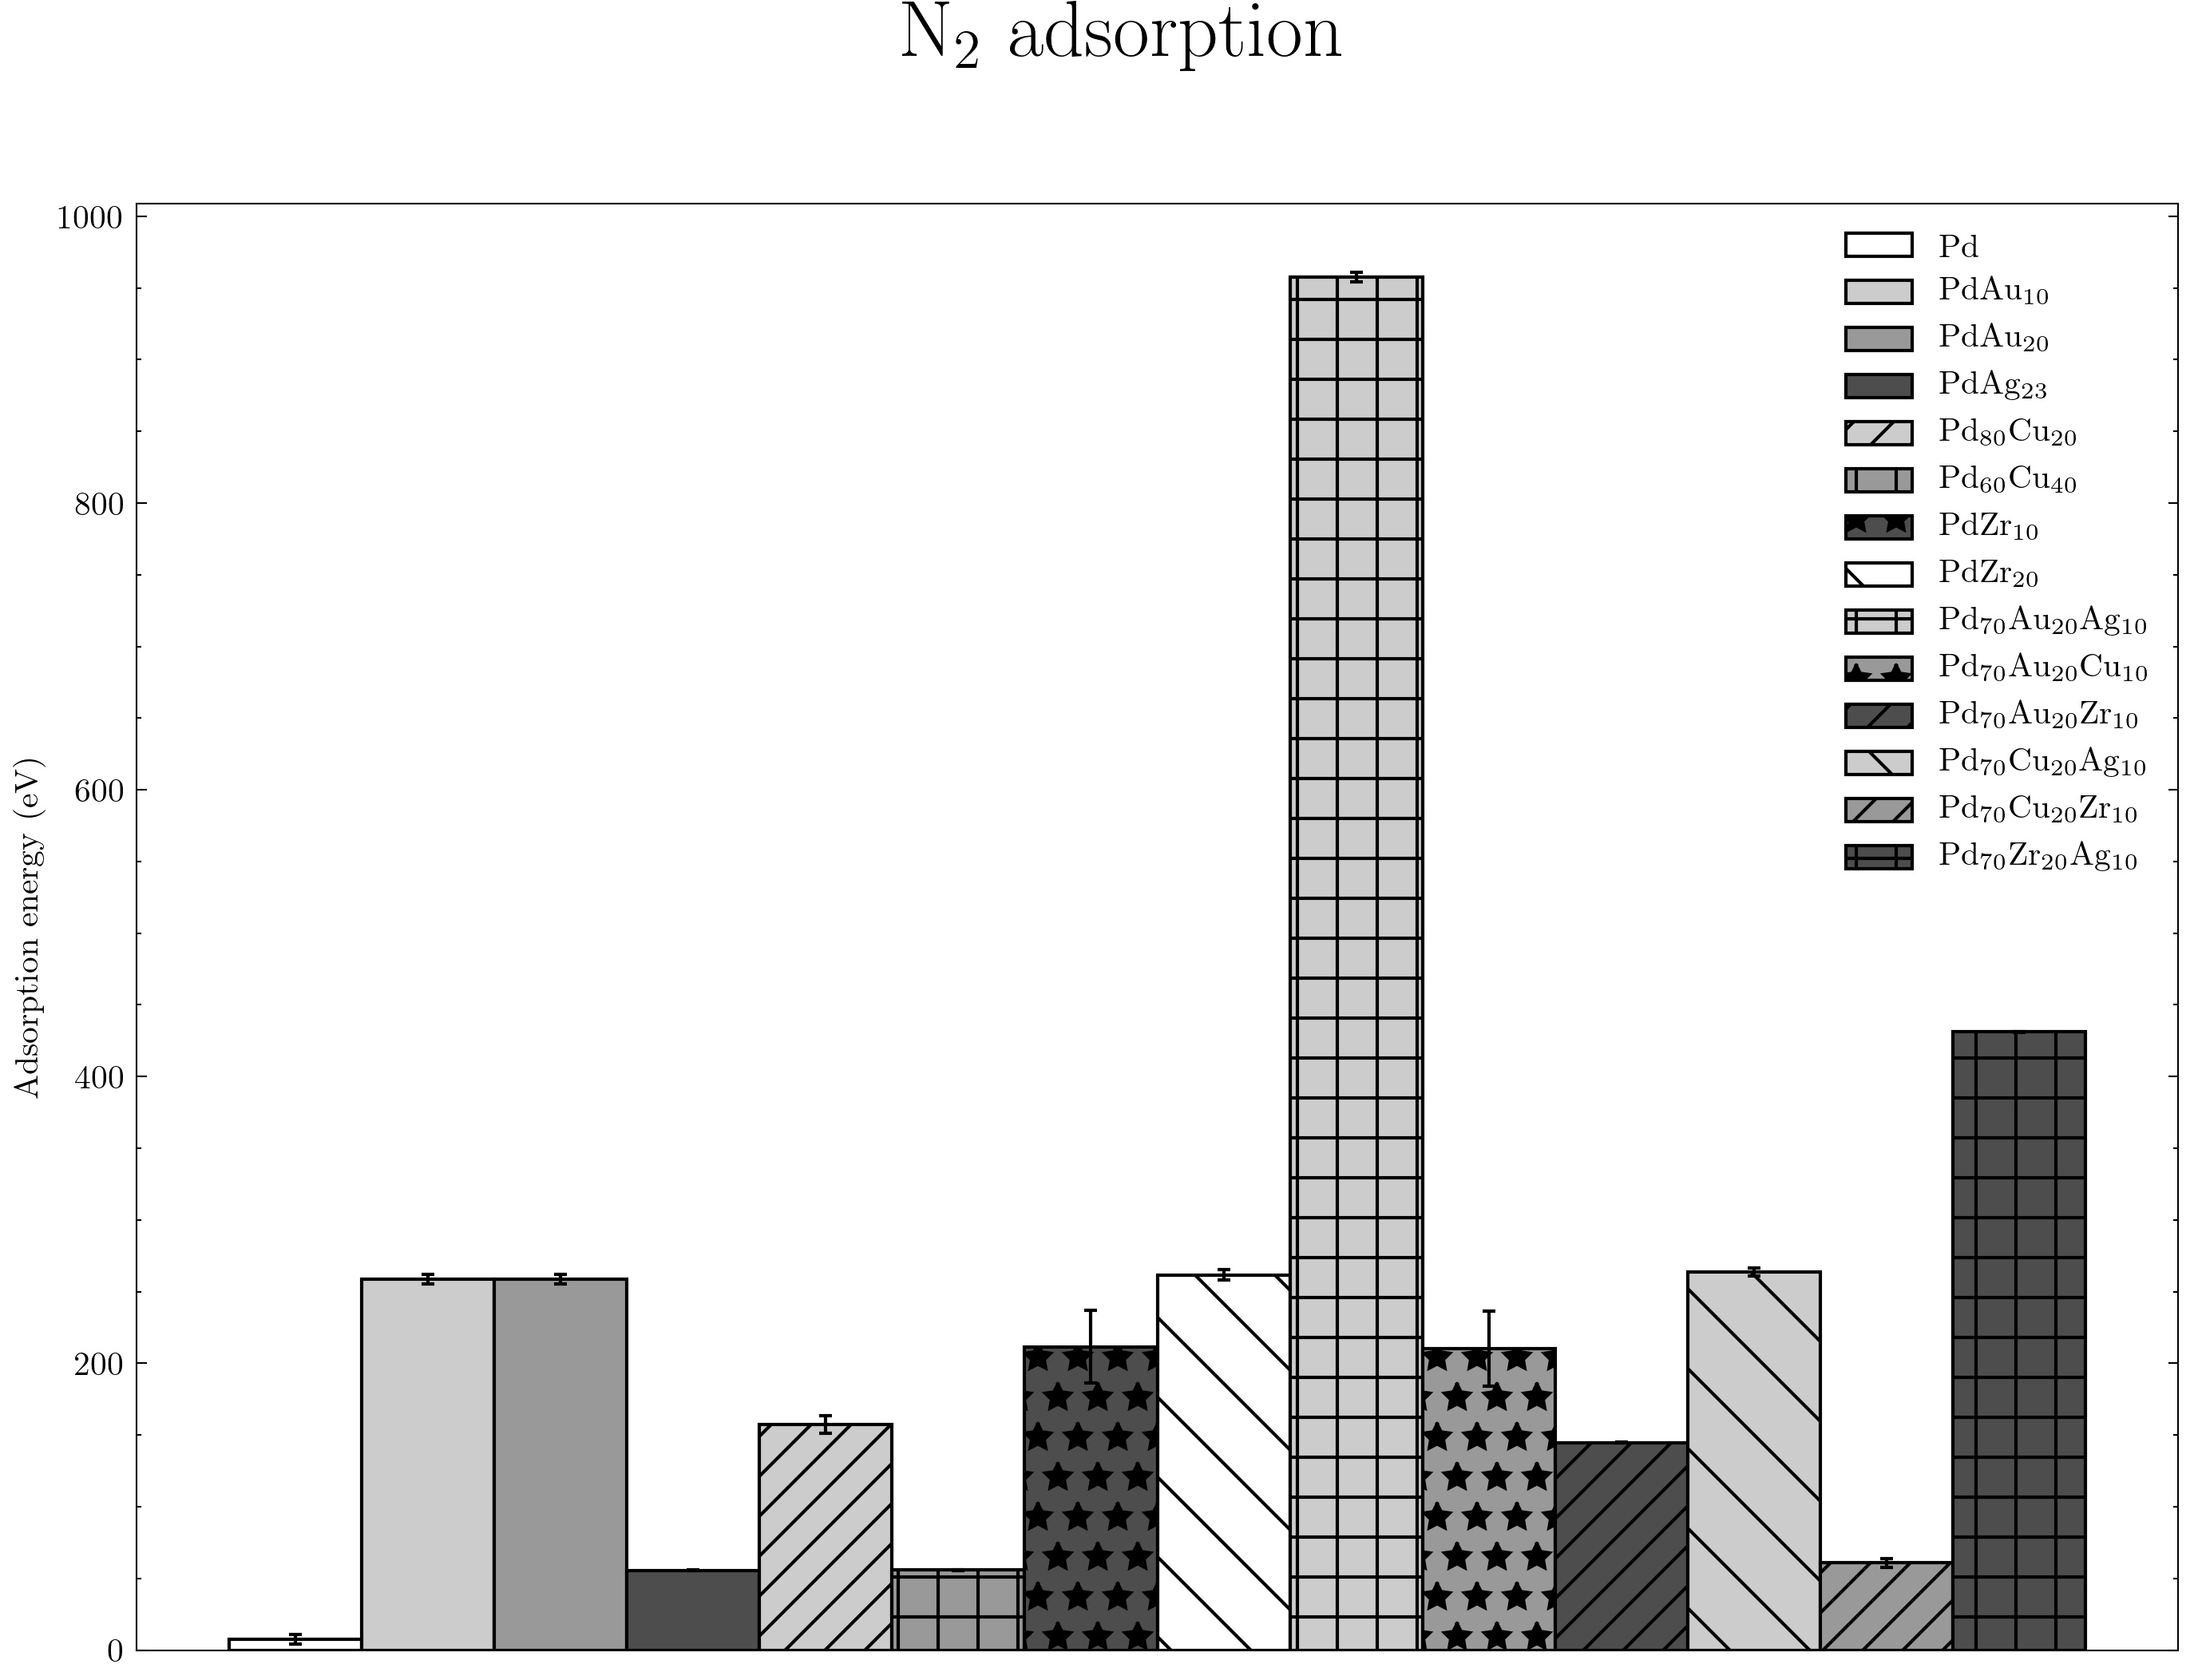
\includegraphics[width=0.9\linewidth, keepaspectratio]{/Users/marc/Thesis/Chapter3/data/N2ads.jpg}
        \caption{Average adsorption energy of N\textsubscript{2} on the surface of palladium and palladium alloy slabs}
        \label{n2ads}
      \end{figure}

    \begin{figure}
        \centering
        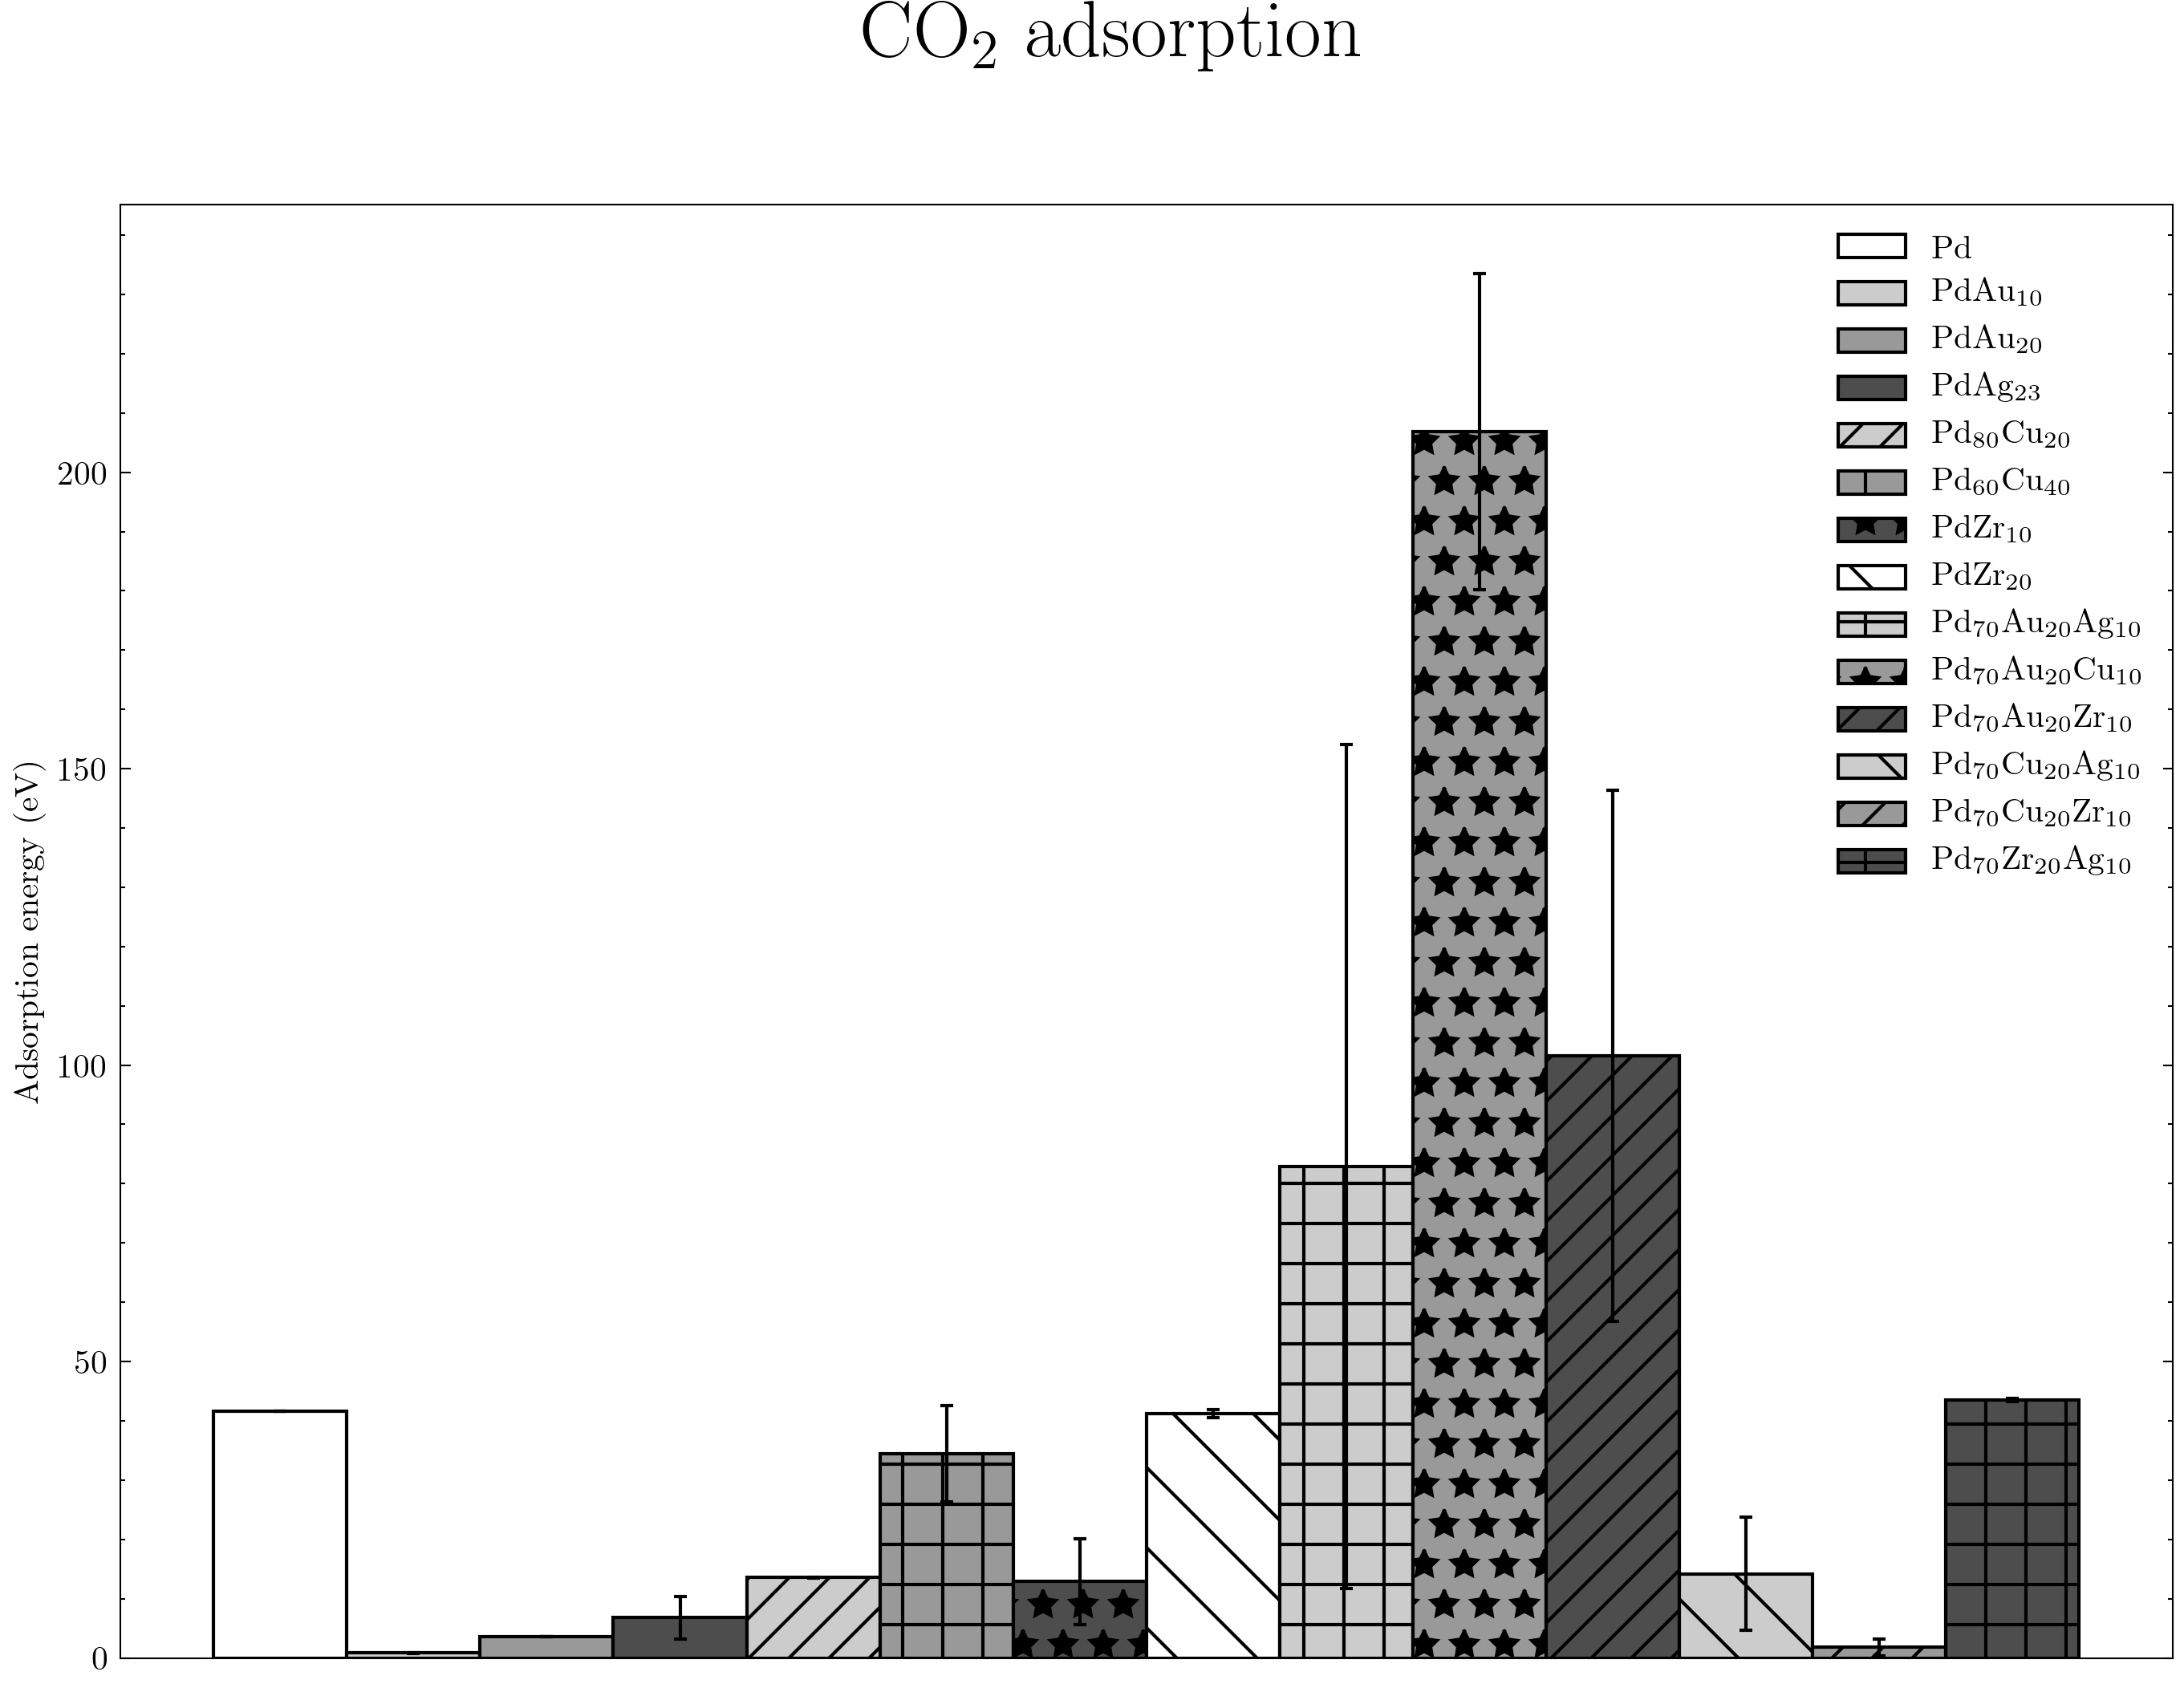
\includegraphics[width=0.9\linewidth, keepaspectratio]{/Users/marc/Thesis/Chapter3/data/CO2ads.jpg}
        \caption{Average adsorption energy of CO\textsubscript{2} on the surface of palladium and palladium alloy slabs}
        \label{co2ads}
      \end{figure}
    
        \begin{figure}
            \centering
            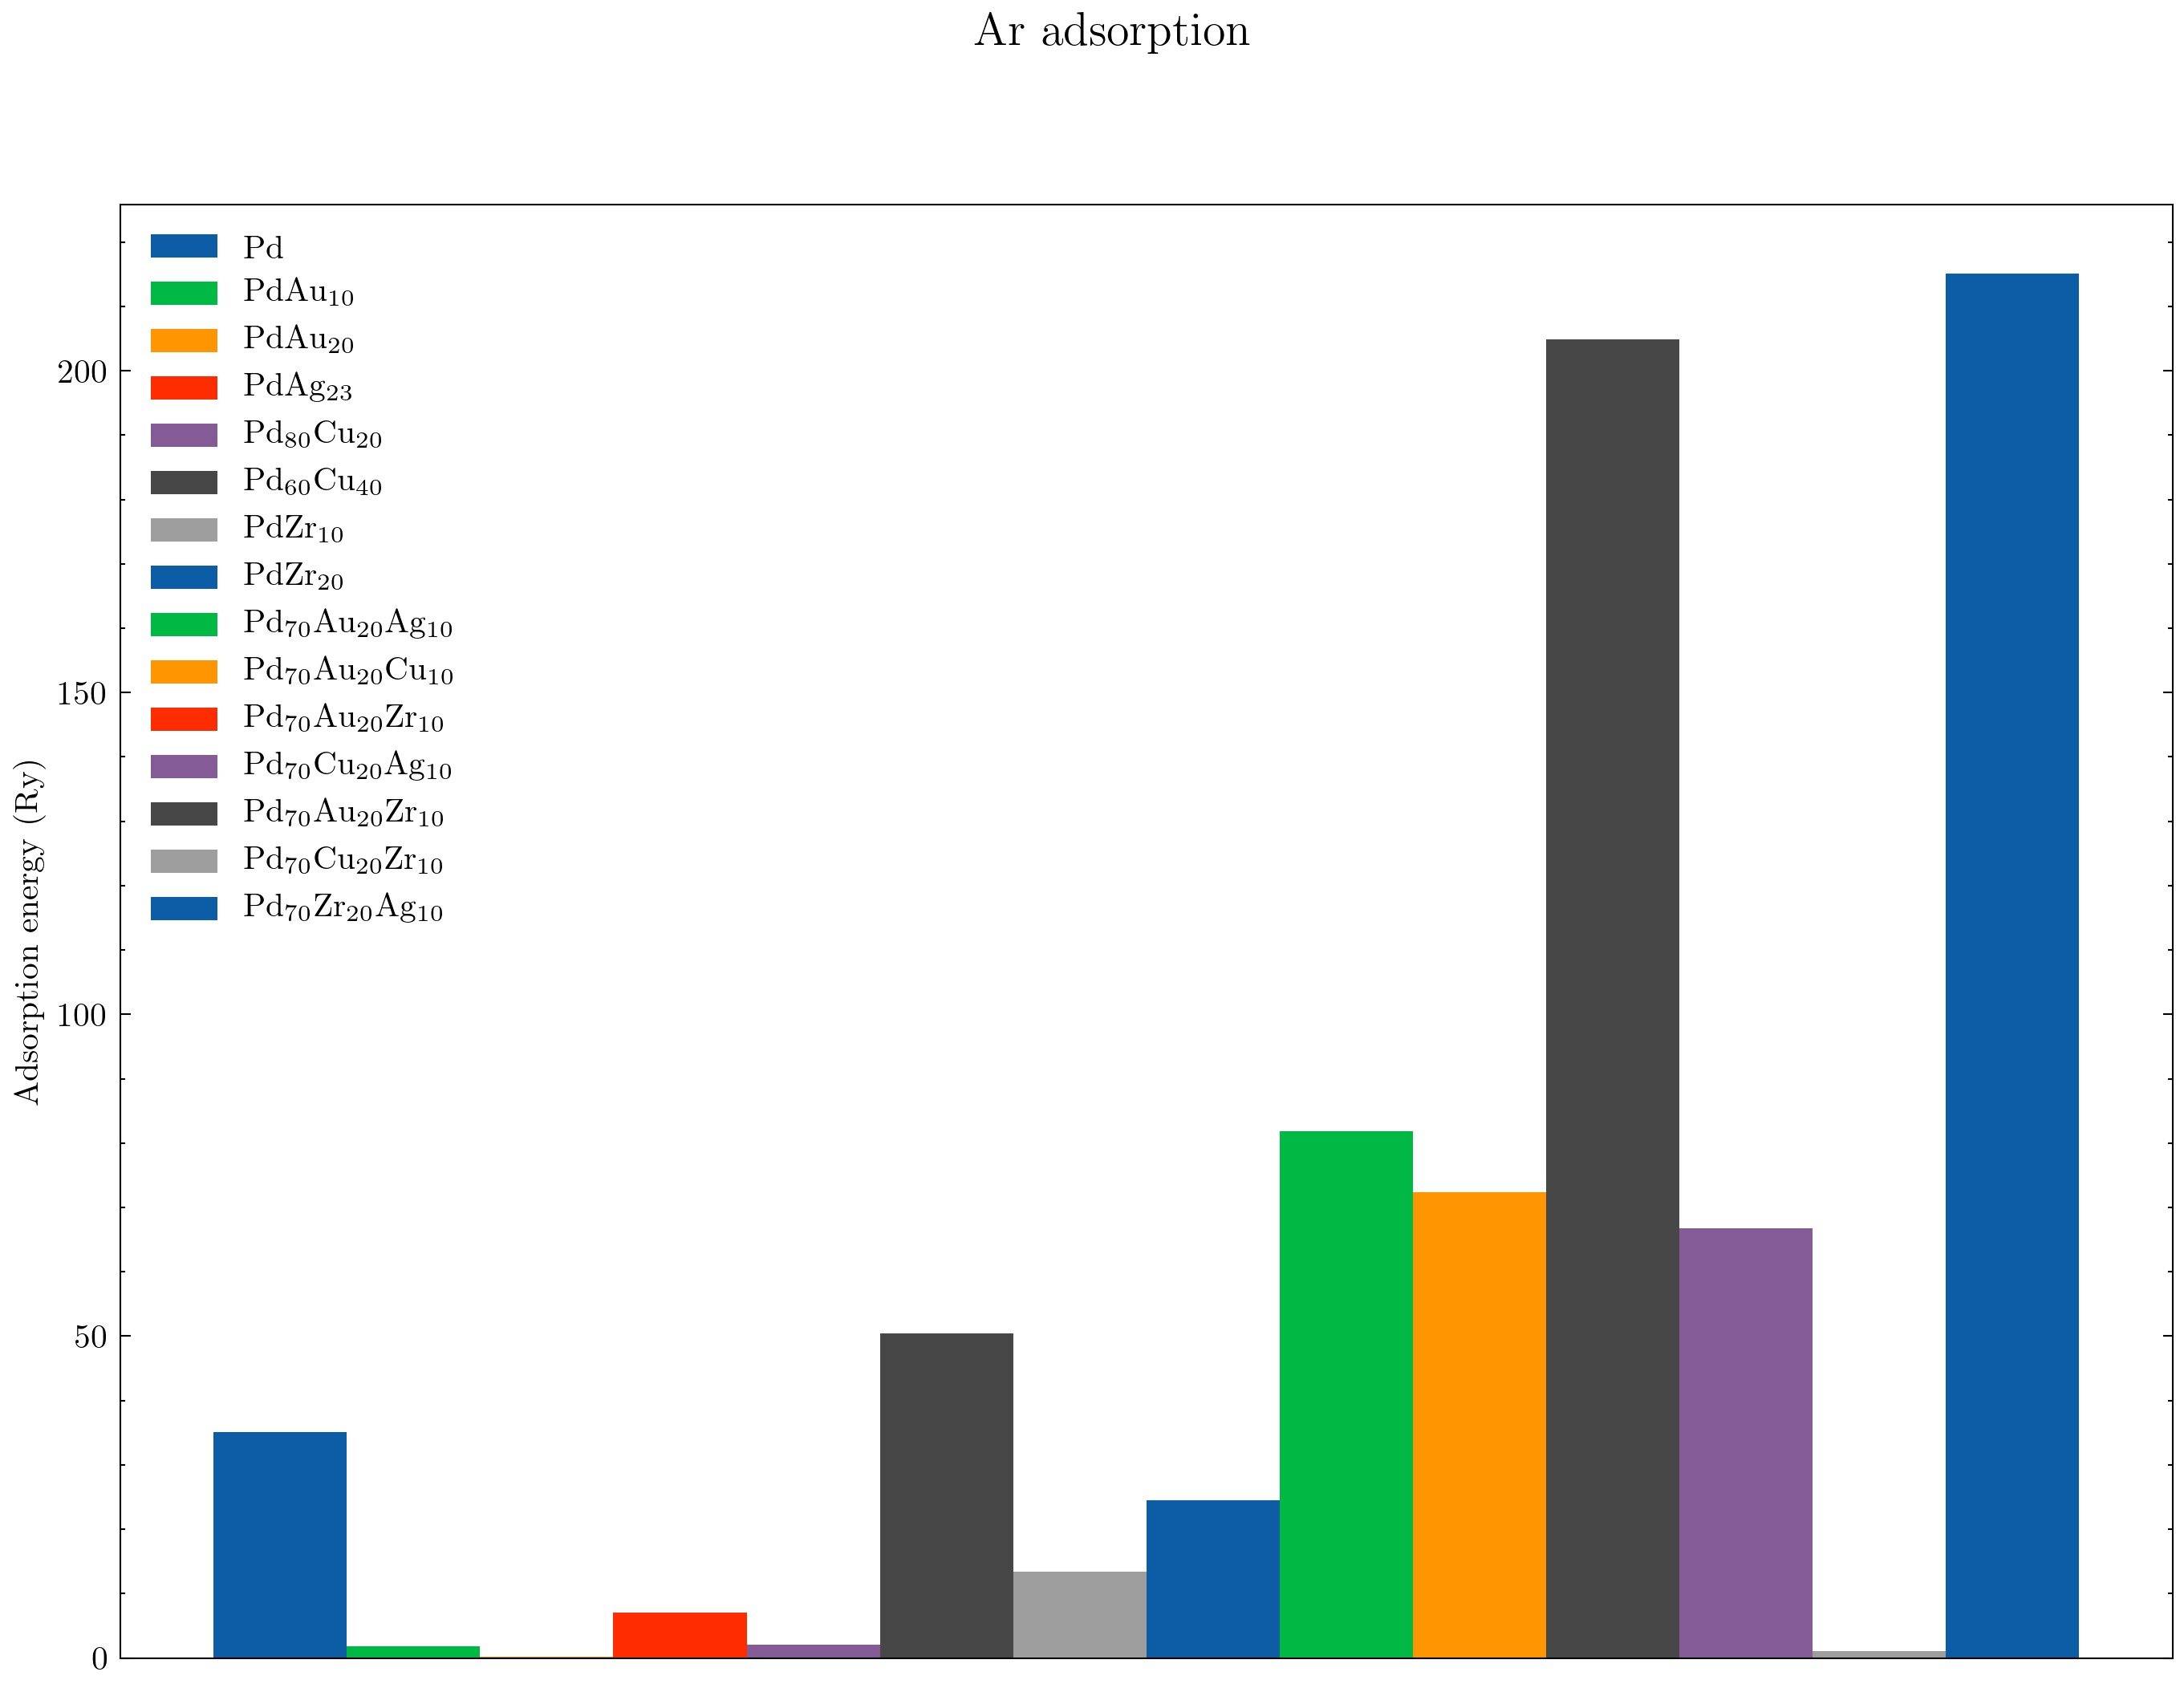
\includegraphics[width=0.9\linewidth, keepaspectratio]{/Users/marc/Thesis/Chapter3/data/ARads.jpg}
            \caption{Average adsorption energy of Ar on the surface of palladium and palladium alloy slabs}
            \label{Arads}
          \end{figure}
        
\subsubsection{Carbon Monoxide}
CO adsorption was performed by adsorbing the gaseous molecule by the C atom as is normal for CO adsorption on metallic surfaces \cite{doi:10.1021/acscatal.8b02371}. All palladium slab systems showed adsorption affinity to CO. The results of the simulations and their adsorption energies compared to that of hydrogen on the same alloy are shown in figure \ref{coads}.  No alloys showed an aversion to CO adsorption therefore all of the simulated alloys, regardless of their Preference to H\textsubscript{2} adsorption, will likely expereince some competitive adsorption and therefore inhibition of flux when CO is present. 

The pure Pd system showed a clear preference to CO adsorption over hydrogen, this matches previous experiments performed to investigate this. \cite{Xu2016a} Figure \ref{COsite} shows the adsorption energy on each site compared to that of H calculated in section \ref{Hsection}. The fcc system shows a clear preference for CO on the FCC, HCP and TOP sites, while still preferring to adsorb H on the BRIDGE site. This is most prevalent for the FCC site which has a lower adsorption energy of around -0.55 eV, with HCP and TOP sites showing a drop in around -0.35 and -0.3 eV respectivley. However since the top site still shows a preference for H adsorption which represents around 41\% of the adsorption sites. While this may indicate that these sites are still avaliable for hydrogen permeation, when bulk diffusion is modelled using kinetic monte carlo simulations that hydrogen travels through the bulk by relaxing the lattice around the fcc and hcp sites to facilitate transport. \cite{Qin2012} Therefore the blocking of these sites is likely to have a severe effect on hydrogen permeation.

Of the systems tested PdAu\textsubscript{20}, PdAg\textsubscript{23}, and Pd\textsubscript{70}Au\textsubscript{20}Cu\textsubscript{10} all showed marginal preference for hydrogen adsorption over CO adsorption. Adsorption of CO on Au and Ag surfaces has previously been studied and concluded that these metals do not interact with CO under normal circumstances, and will only adsorb through way of material defect or alloying. \cite{doi:10.1021/la950167j} \cite{shaikhutdinov_meyer_naschitzki_baumer_freund_2003}

By far the worst performing metal for inhibiting the effect of CO were all Zr containing alloys, and Pd\textsubscript{60}Cu\textsubscript{40}. Zr readily forms a bond with C, and even has it's own unique branch of chemistry referring to such compounds.\cite{doi:10.1021/cen-v082n016.p036} Zirconium is also a common complex used in homogeneous refactory catalysts for reforming hydrocarbon compounds.\cite{doi:10.1002/9780470504437.ch1} Therefore the evidence suggests that Zr naturally has a high affinity towards forming carbon bonds and is not a suitable additive for CO resistent membranes. 

Similarly Cu has been previously studied and found to readily adsorb CO on it's surface. \cite{doi:10.1021/la950167j} This does not appear to be an issue for PdCu\textsubscript{20} alloys. The Pd\textsubscript{60}Cu\textsubscript{40} alloy on the other hand has a much higher binding energy than it's sister hydrogen system. Pd\textsubscript{60}Cu\textsubscript{40} is different from other systems in that the crystalline structure transitions to a BCC lattice. \cite{She2014} BCC structures only have two different sites avaliable for hydrogen adsorption, BRIDGE and HCP. \cite{C3CP44367A} This change in structure combined with the Cu's avalability to bind with C likely accounts for the large discrepancy. 

\begin{figure}
  \centering
  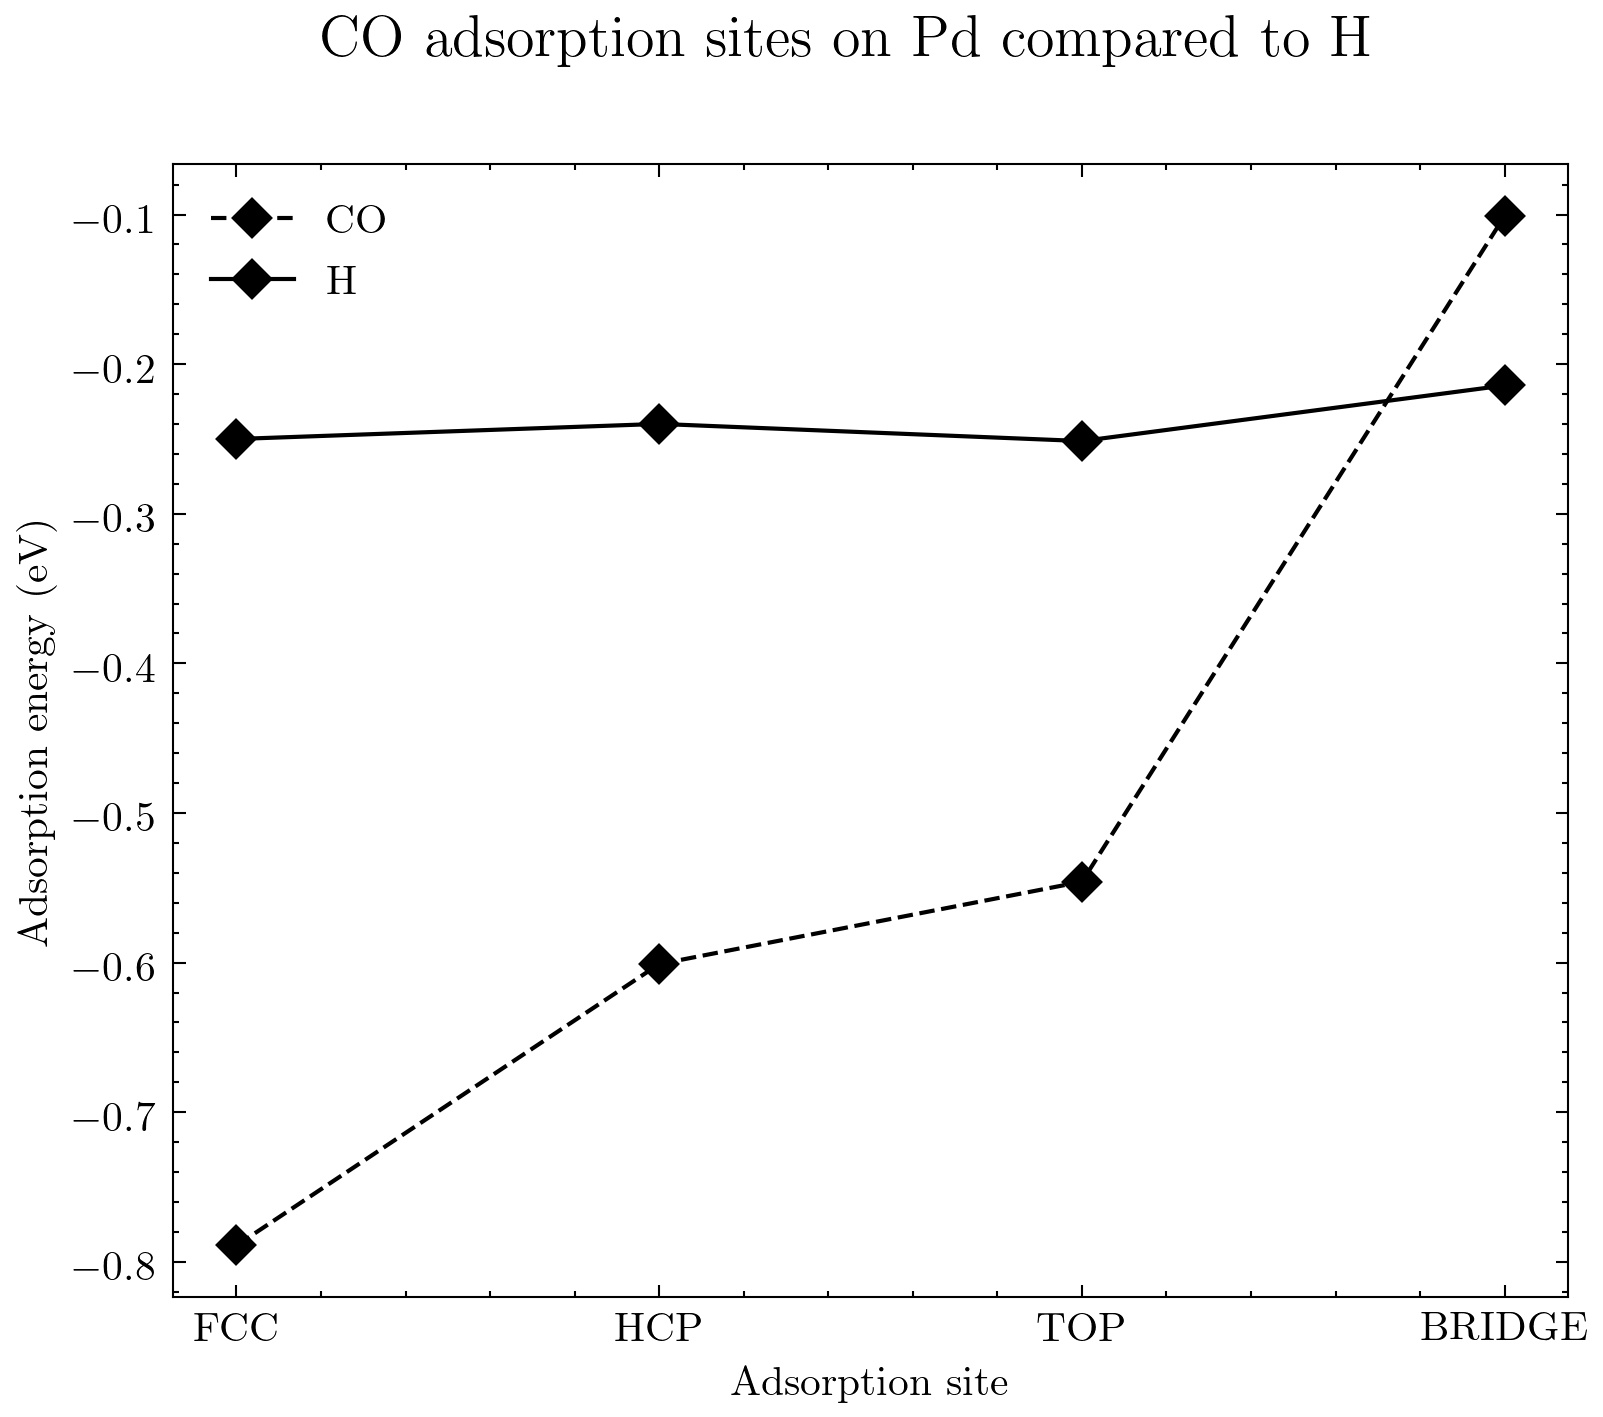
\includegraphics{/Users/marc/Thesis/Chapter3/data/COSites.jpg}
  \caption{Adsorption energy of H for each site on a 2x2x5 Pd slab}
  \label{COsite}
\end{figure}


\begin{landscape}
    \begin{figure}
        \centering
        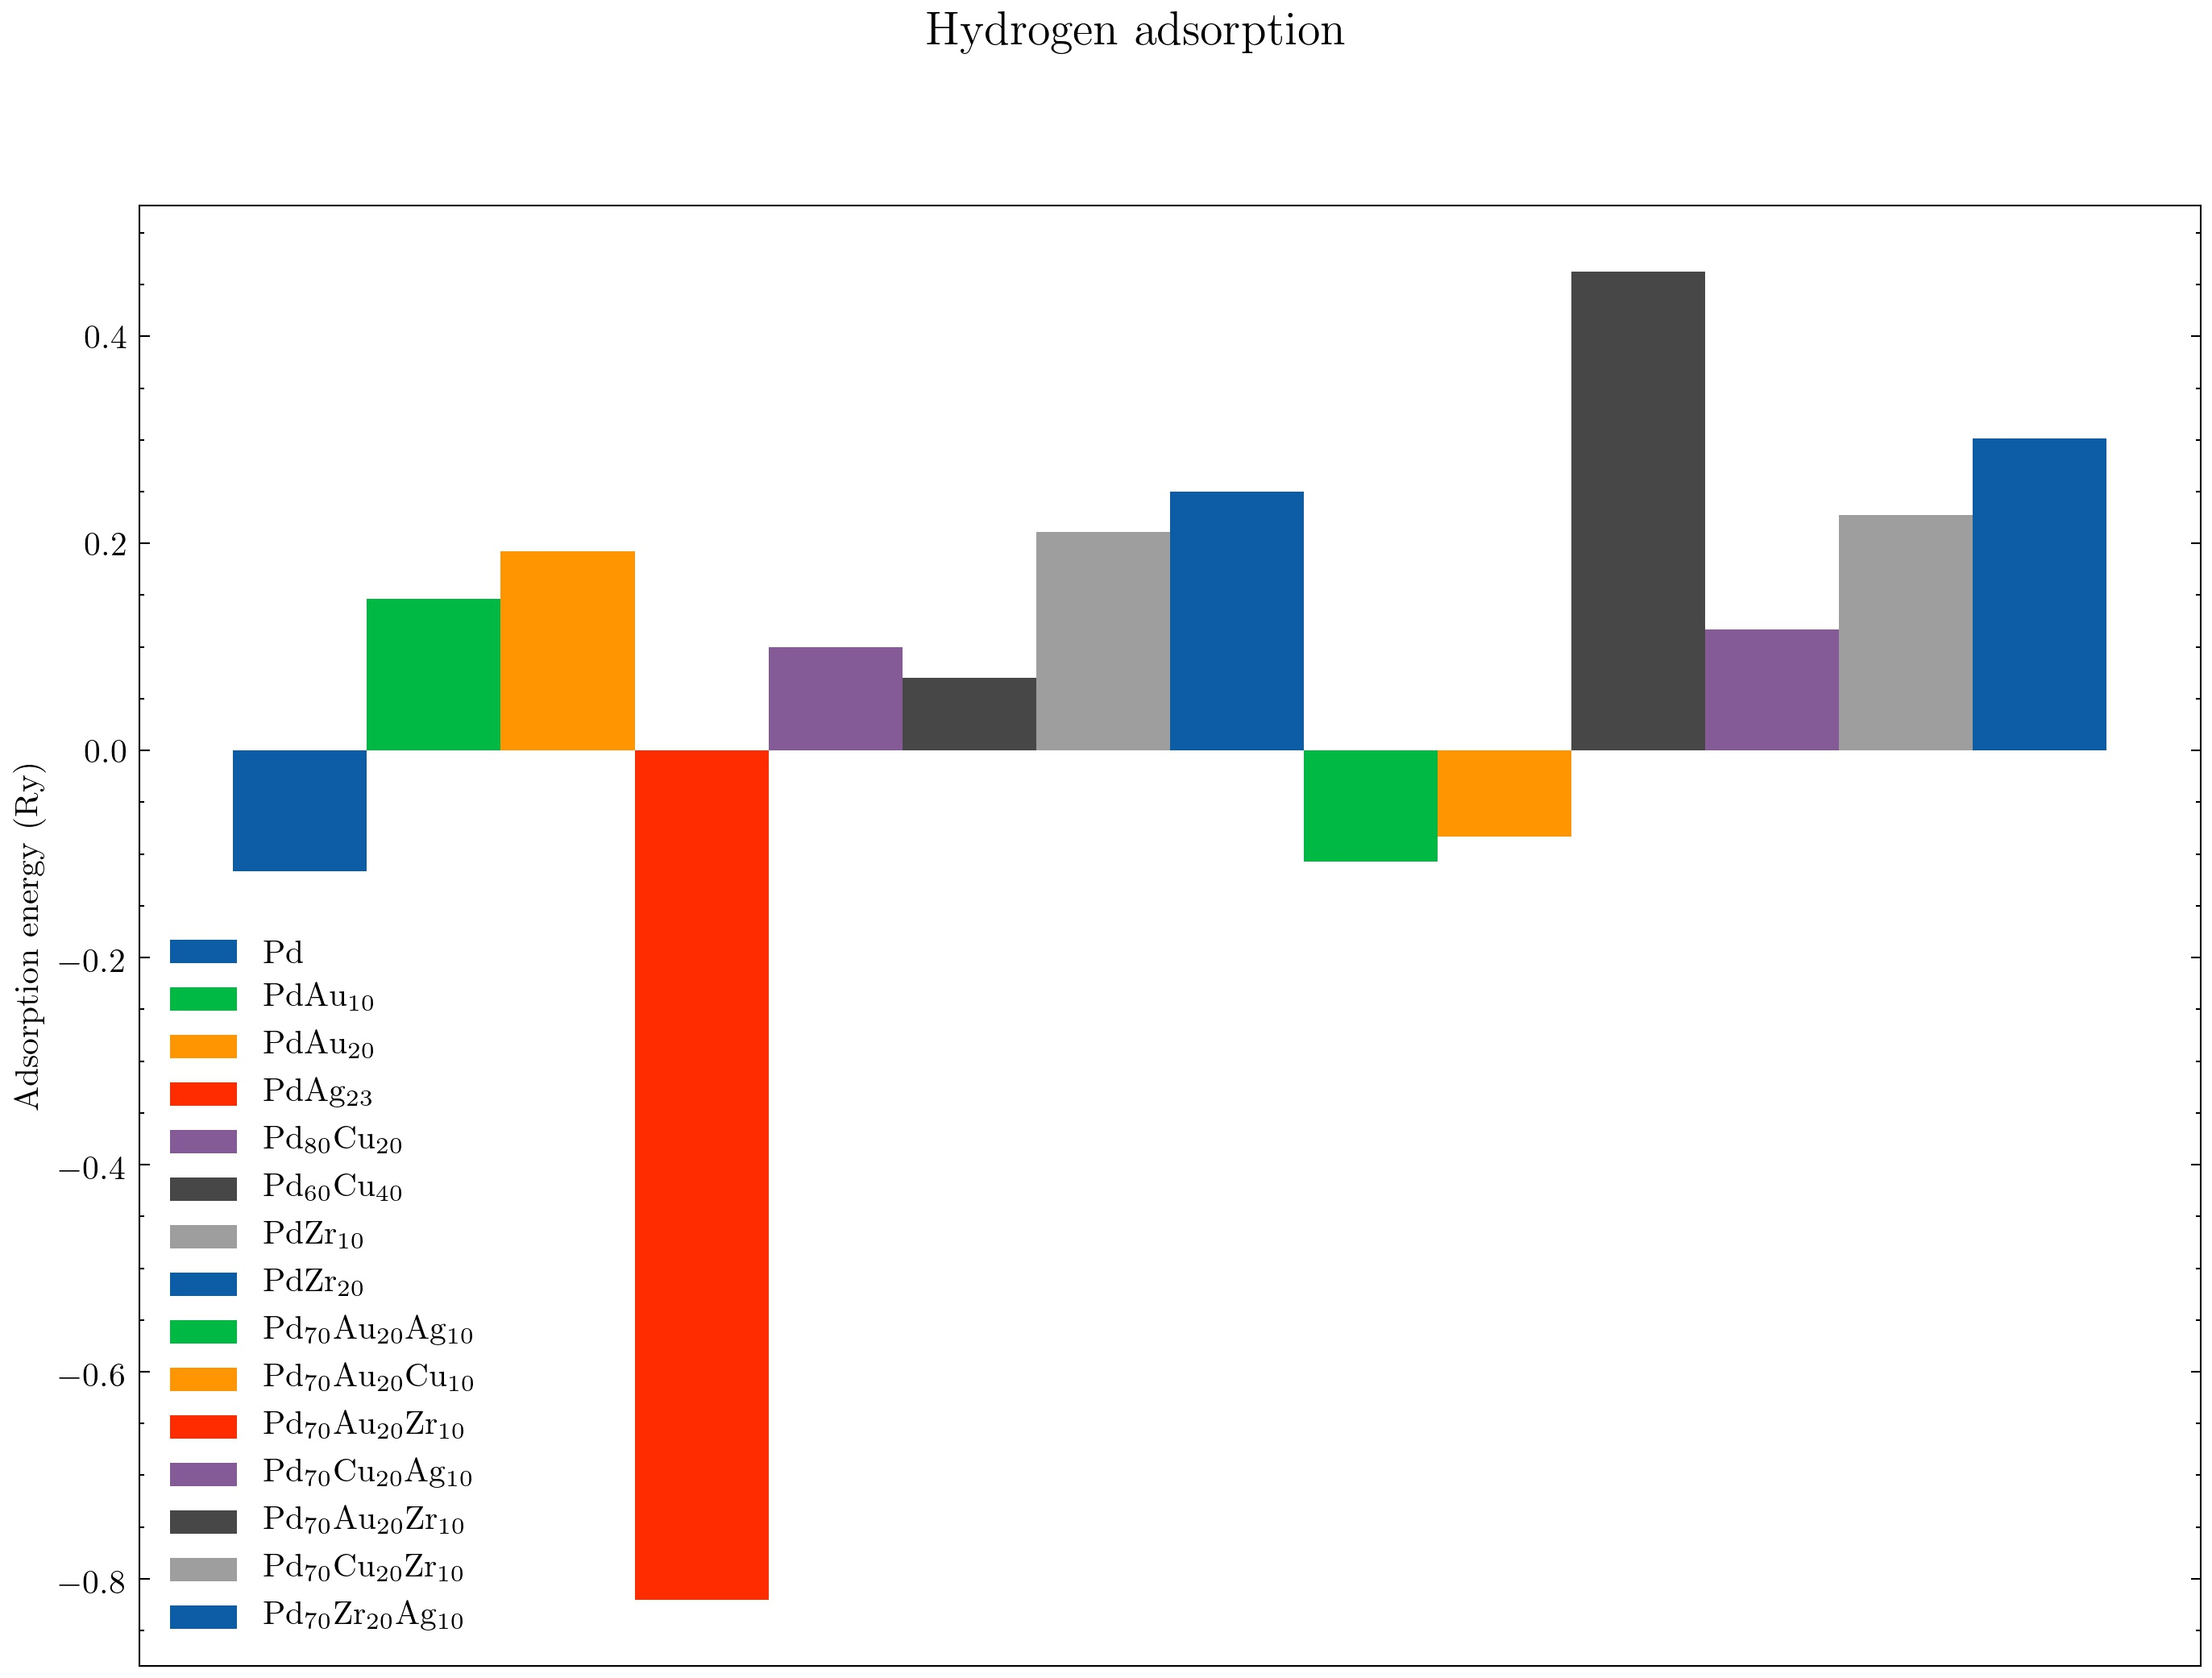
\includegraphics[width=0.9\linewidth,height=\textheight, keepaspectratio]{/Users/marc/Thesis/Chapter3/data/COads.jpg}
        \caption{Average adsorption energy of CO on the surface of palladium and palladium alloy slabs}
        \label{coads}
      \end{figure}
    
    \end{landscape}
\subsubsection{Ammonia}
The results of the ammonia simulations on the palladium alloy slabs are shown in figure \ref{nh3ads}. Of the tested material compositions, neither palladium or any alloy showed an ability to readily bind with Ammonia, this was also true across all sites on the fcc and bcc lattice. This is consistent with the experimental results of Lundin et al \cite{Lundin2016} and the previous simulations by Herron et al \cite{HERRON20121670}. It should be noted that the paper by Herron \cite{HERRON20121670} found that while ammonia itself did not bind with the surface of palladium, radicals which can be created from ammonia such as imidogen (NH) and azanide (NH\textsubscript{2}) will readily form bonds. It is however extremely unlikely that these compounds wil be present in fuel cell hydrogen, and in the unlikely event they are they will likely instantly reform into the more stable NH\textsubscript{3}. It can be concluded therfore that NH\textsubscript{3} will create no challenges for the operation of palladium membranes. 

  \begin{figure}
      \centering
      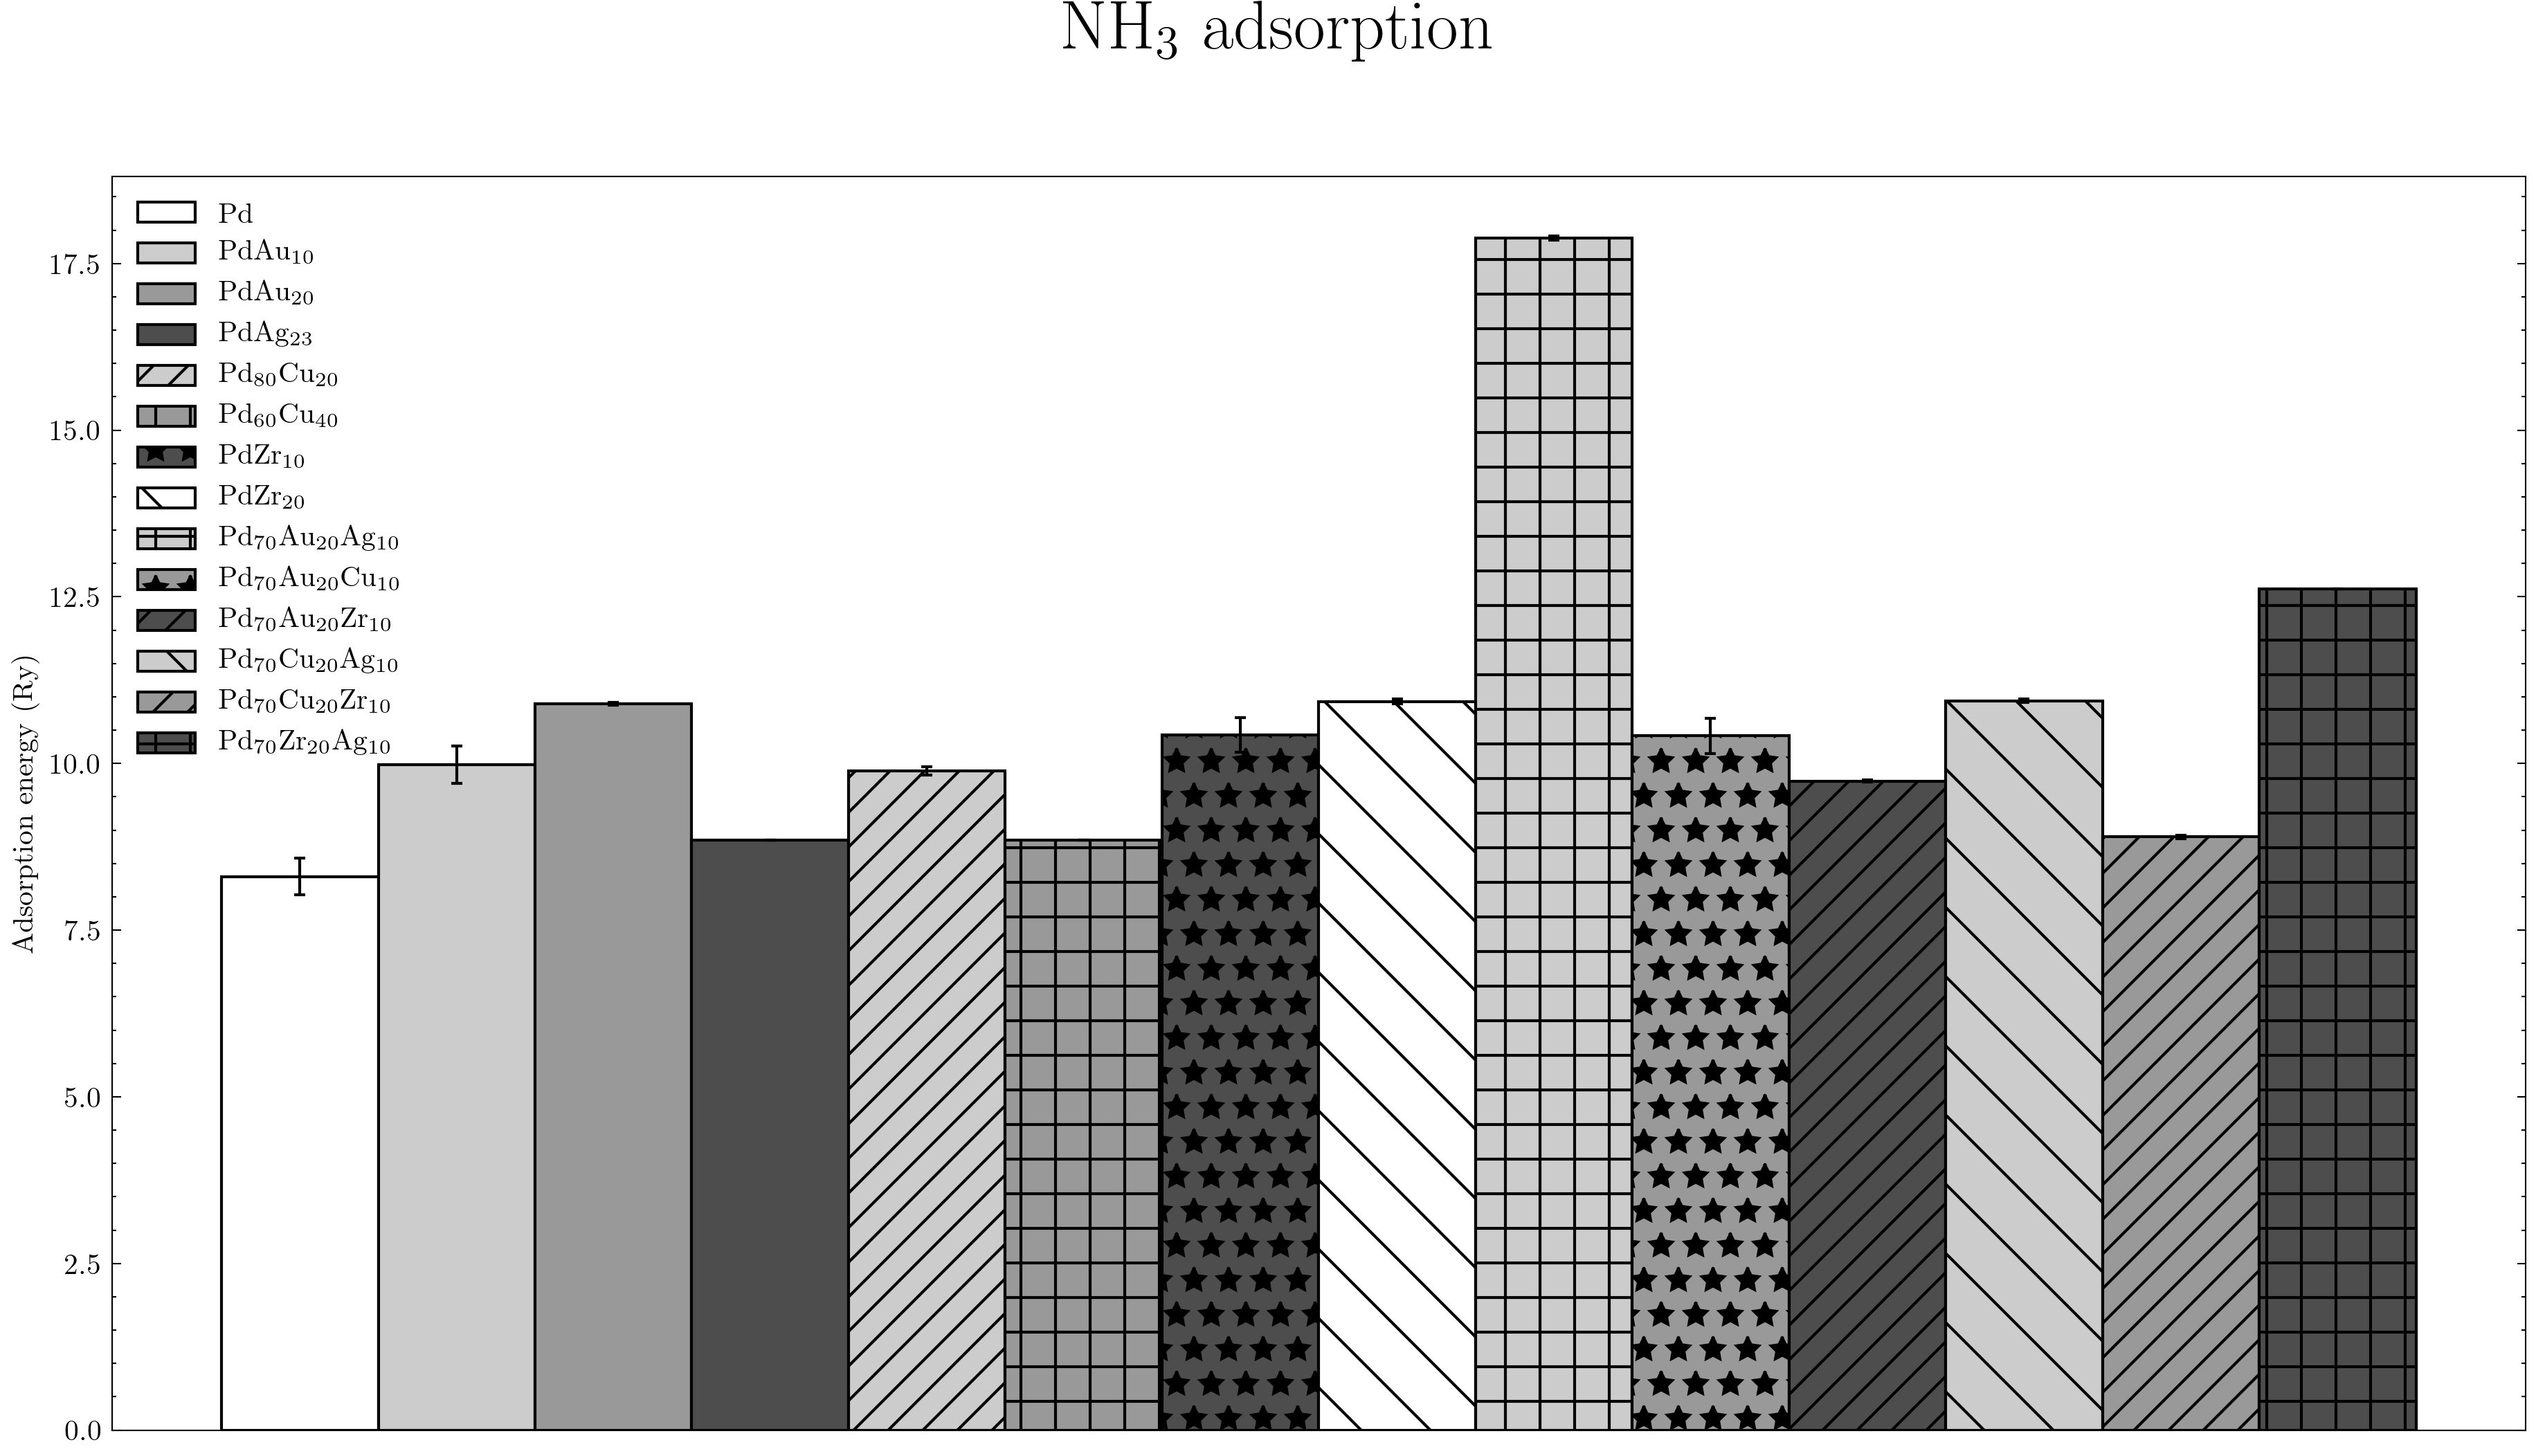
\includegraphics[width=0.9\linewidth,height=\textheight, keepaspectratio]{/Users/marc/Thesis/Chapter3/data/NH3ads.jpg}
      \caption{Average adsorption energy of NH\textsubscript{3} on the surface of palladium and palladium alloy slabs}
      \label{nh3ads}
    \end{figure}
  
\subsubsection{Oxygen and Water}
Since O\textsubscript{2} is a symetrical molecule adsorption was performed similarly to H\textsubscript{2} in section \ref{Hsection}, the results of which are shown in figure \ref{O2ads}. Alloys consisting mainly of noble metals (Pd, Ag, Au) typically did not readily bind with oxygen. Whereas metals which do (Zr and Cu) showed an affinity towards oxygen binding. This can pose an issue during enrichment as this adsorption will likely lead to either the formation of oxides on the surface of the membrane, or catalyse a reaction between either oxygen and hydrogen, or oxygen and one of the other gaseous impurities. In the former the formation of oxides creates a shift in the lattice parameter, similar to the $\alpha - \beta$ transition seen in pure palladium membranes (figure \ref{lit-alphabeta})\cite{Li2008b} and cause membrane failure. In the latter results from hydrogen impurity can be thrown off. Therefore if oxygen is expected in the sample Zr and Cu containing alloys should be avoided.

Water adsorptrion was performed by atatching the molecule top each avaliable site as per previous studies. \cite{Roques2009} The results are shown in figure \ref{H2Oads} and follow the same trend as the O\textsubscript{2} results discussed above. One important caveat when considering water adsorption on the surface of metals is the ability for H\textsubscript{2}O molecule to form hydrogen bonds with neighbouring molecules.\cite{PhysRevB.69.195404} While this study only considered the influence of a single water molecule, in real tests the system will likely have a number of water molecules present. The effect of the hydrogen bond would likely result in the further stabilisation of future water molecules onto the surface, creating an exponential increase in adsorbed H\textsubscript{2}O. \cite{PhysRevB.69.195404} Care should also be taken, as previous studies on other metallic systems have shown that the adsorption of water often leads to subsequent dissociation, and formation of a metal oxide and hydrogen. Leading to the same problems with oxidation as previously discussed. \cite{doi:10.1021/jz300994e}

In conclusion noble metals appear to be the best alloying compounds to protect against the influence of H\textsubscript{2}O and O\textsubscript{2}. This is to be expected as these metals are traditionally resistant to oxidation. It should be noted however that while this study focused on adsorption of water on the membrane, it does not take into account adsorption on any other components and fittings on a system. Water in particular is notoriously difficult to remove from a system due to it's avaliability for adsorption on metal surfaces.\cite{BACQUART20205565} Therefore while reducing it's effect on the membrane solves one problem, it's effect on the overall system still has to be considered. 

\begin{landscape}
  \begin{figure}
      \centering
      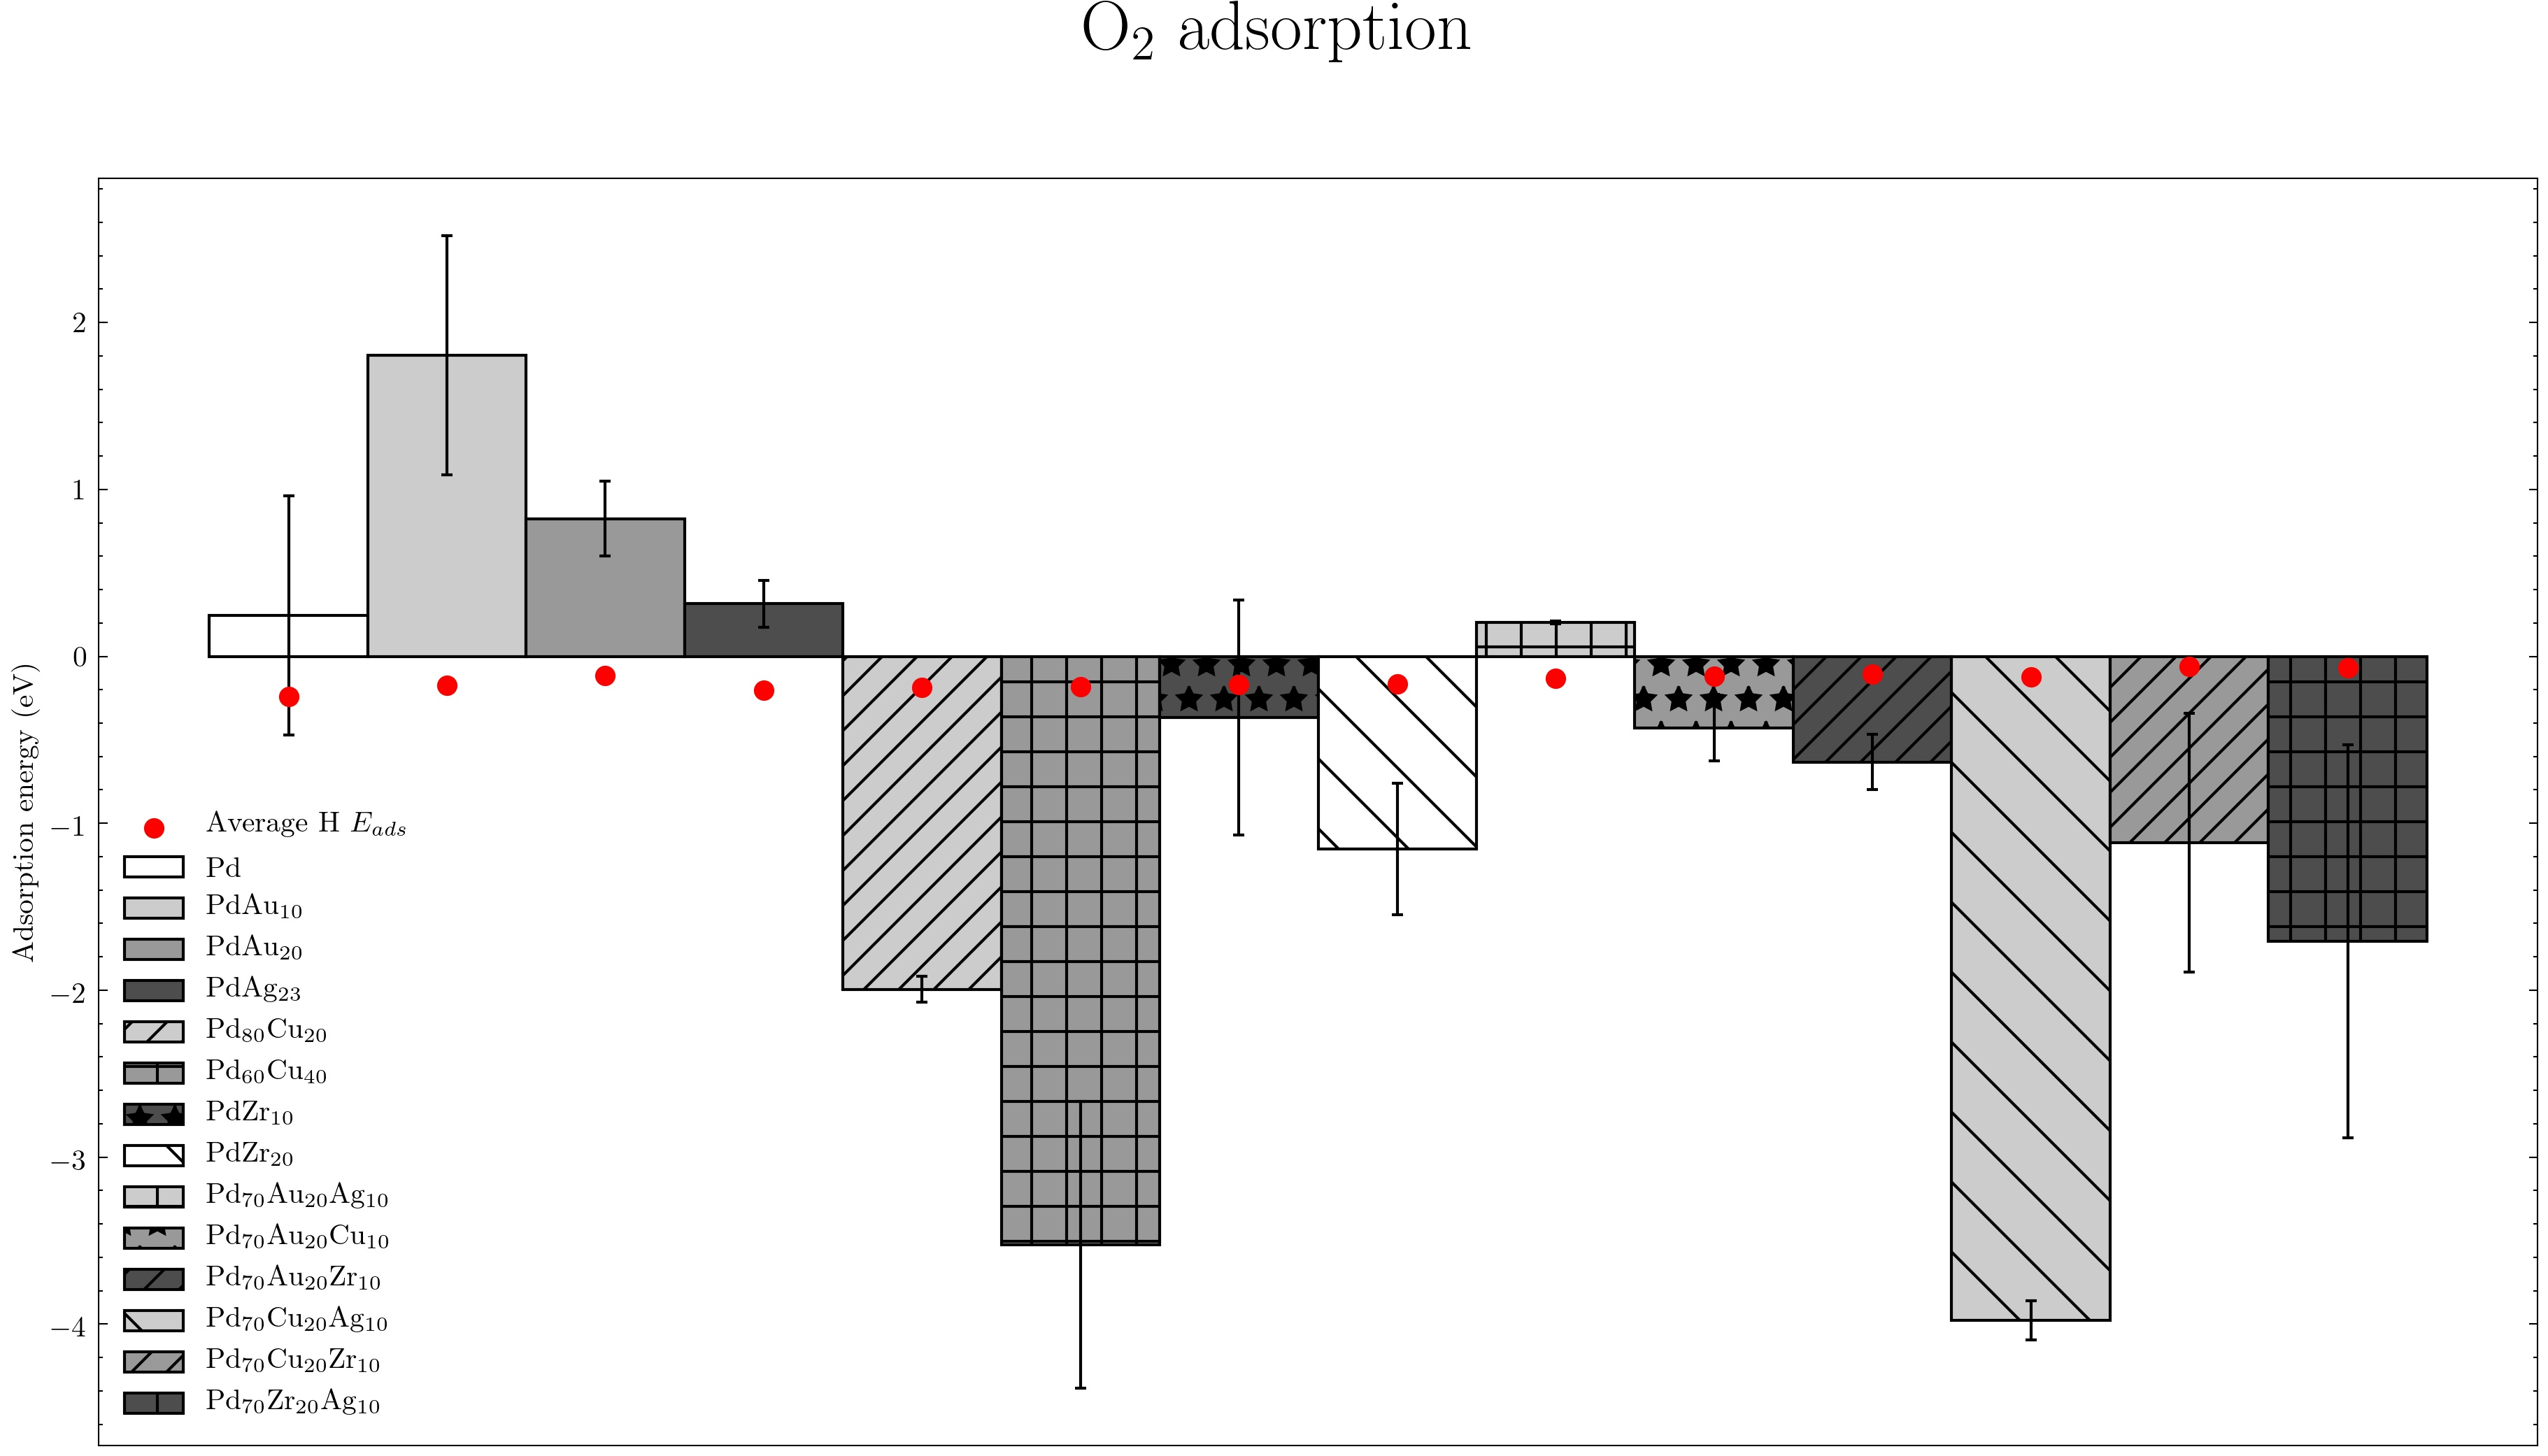
\includegraphics[width=0.9\linewidth,height=\textheight, keepaspectratio]{/Users/marc/Thesis/Chapter3/data/O2ads.jpg}
      \caption{Average adsorption energy of O\textsubscript{2} on the surface of palladium and palladium alloy slabs}
      \label{O2ads}
    \end{figure}
  
  \end{landscape}


\begin{landscape}
  \begin{figure}
      \centering
      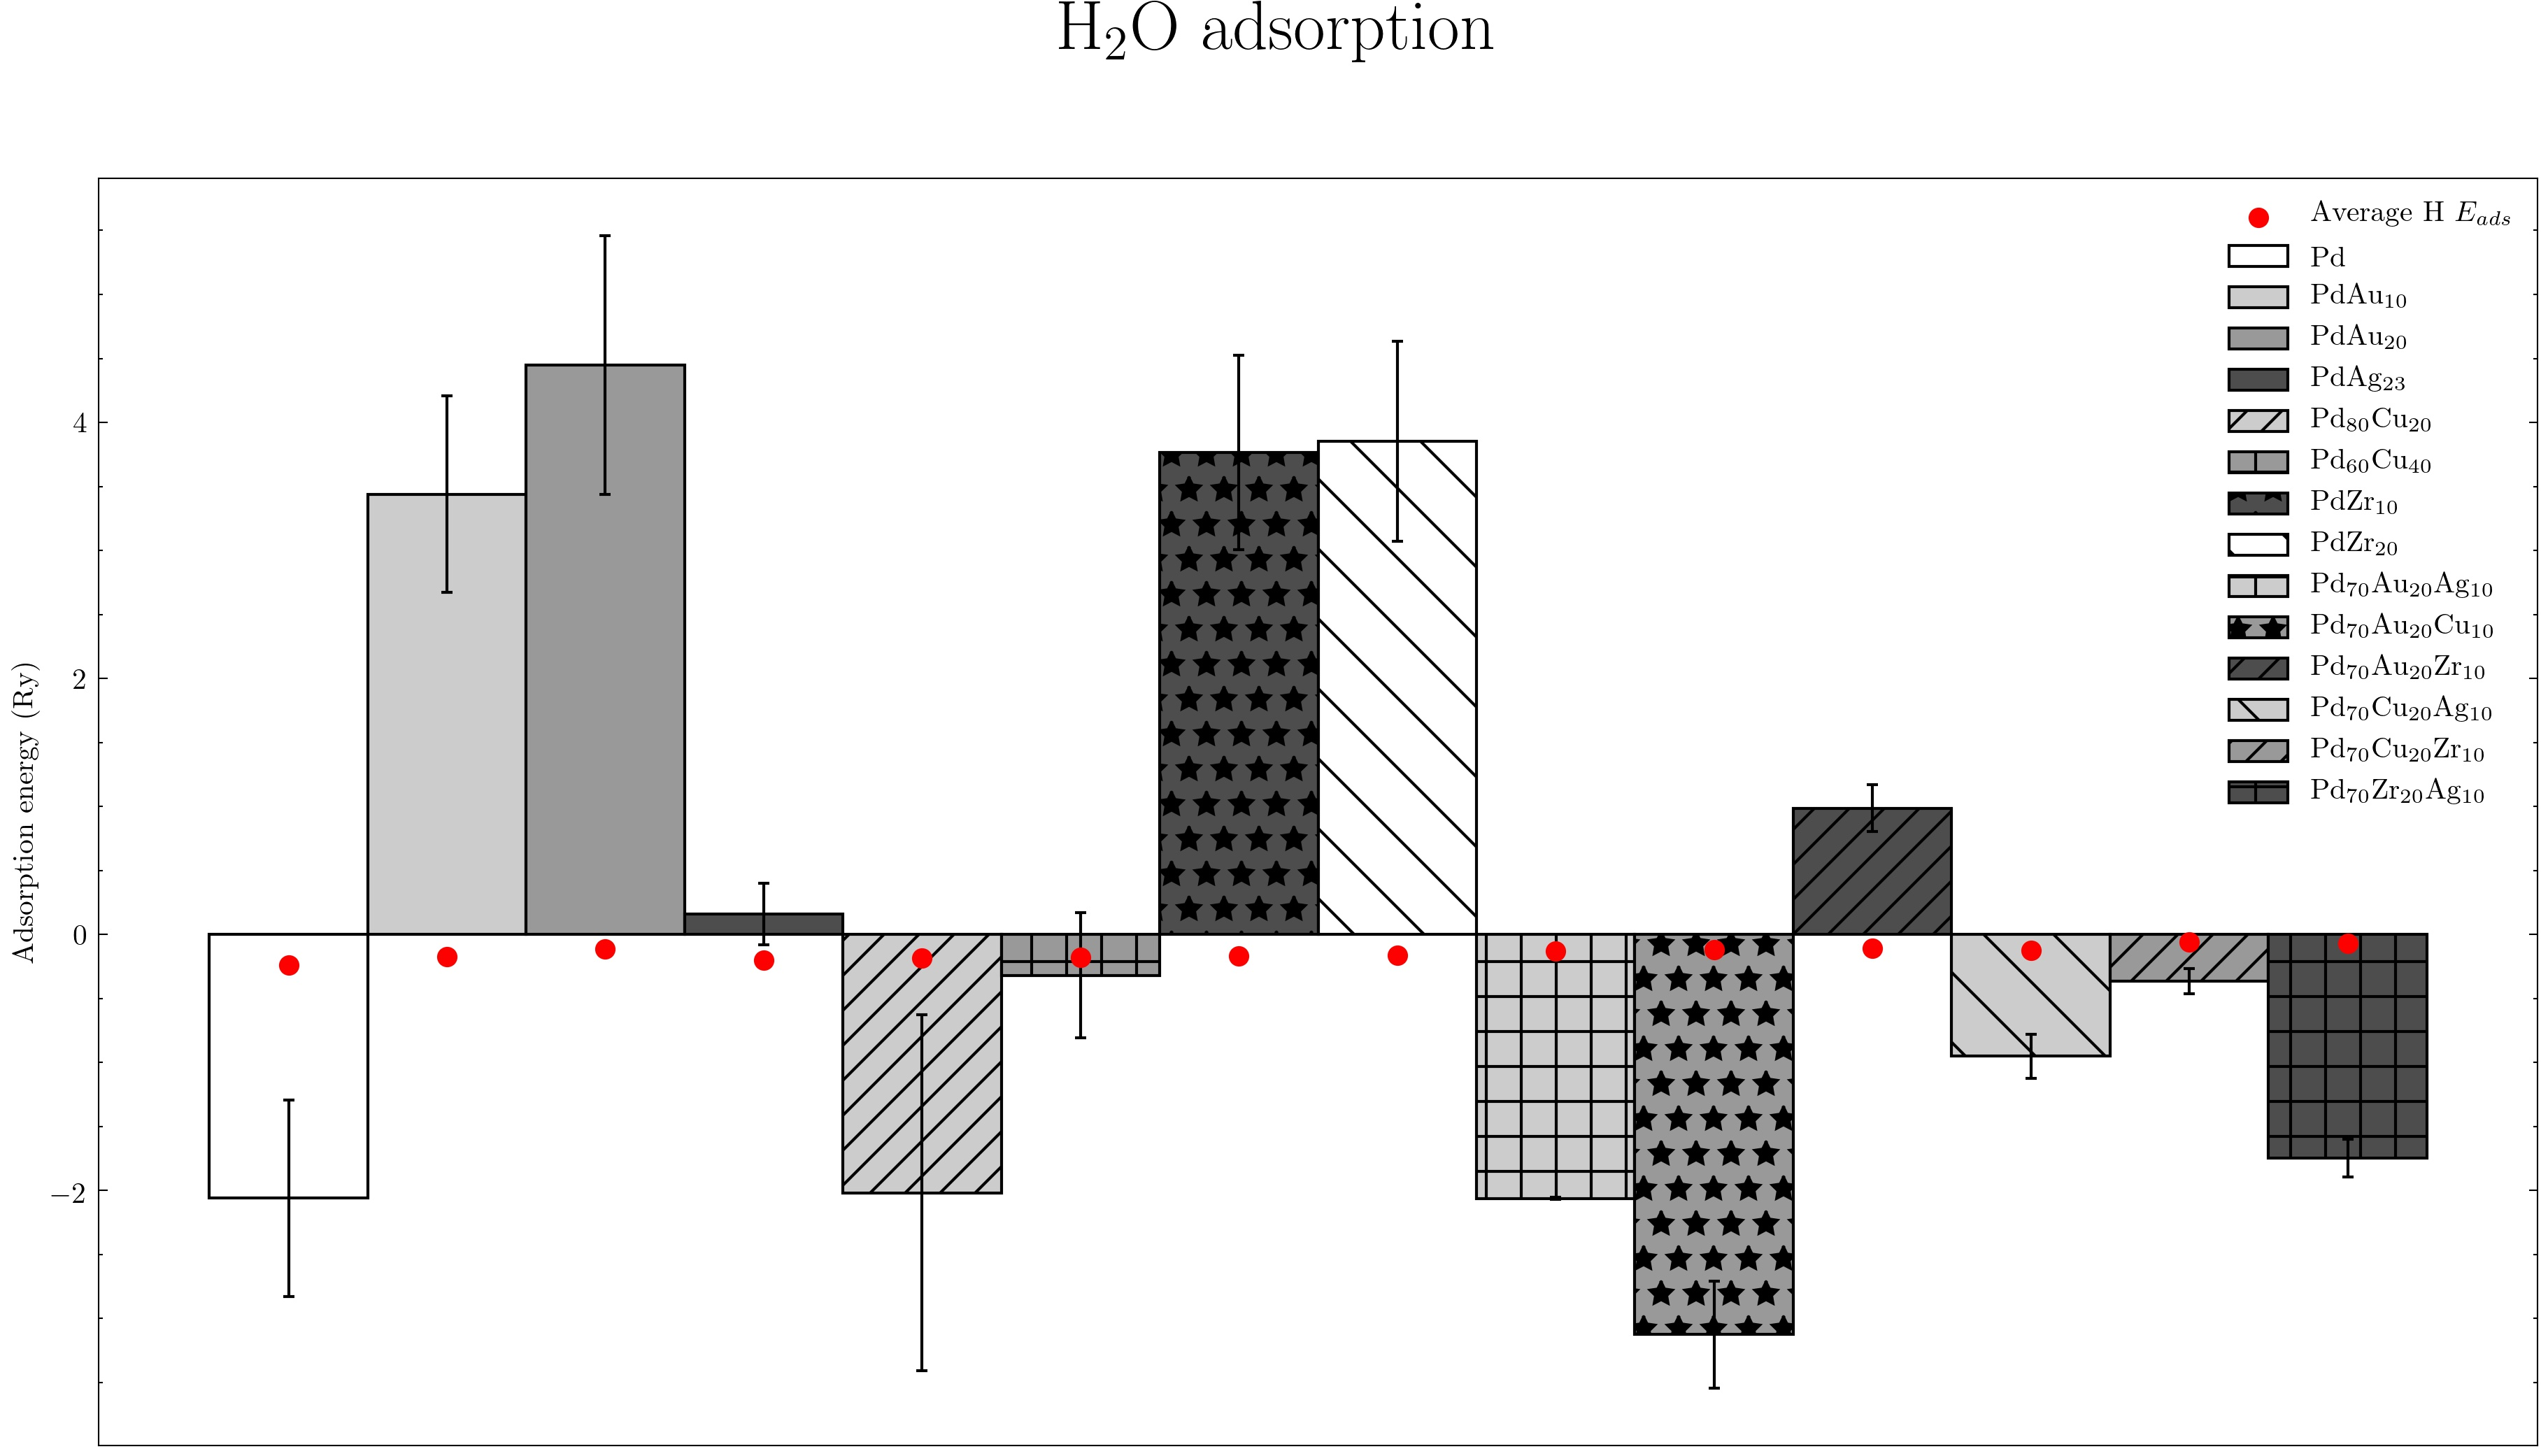
\includegraphics[width=0.9\linewidth,height=\textheight, keepaspectratio]{/Users/marc/Thesis/Chapter3/data/H2Oads.jpg}
      \caption{Average adsorption energy of H\textsubscript{2}O on the surface of palladium and palladium alloy slabs}
      \label{H2Oads}
    \end{figure}
  
  \end{landscape}

\subsubsection{Methane}
\begin{landscape}
  \begin{figure}
      \centering
      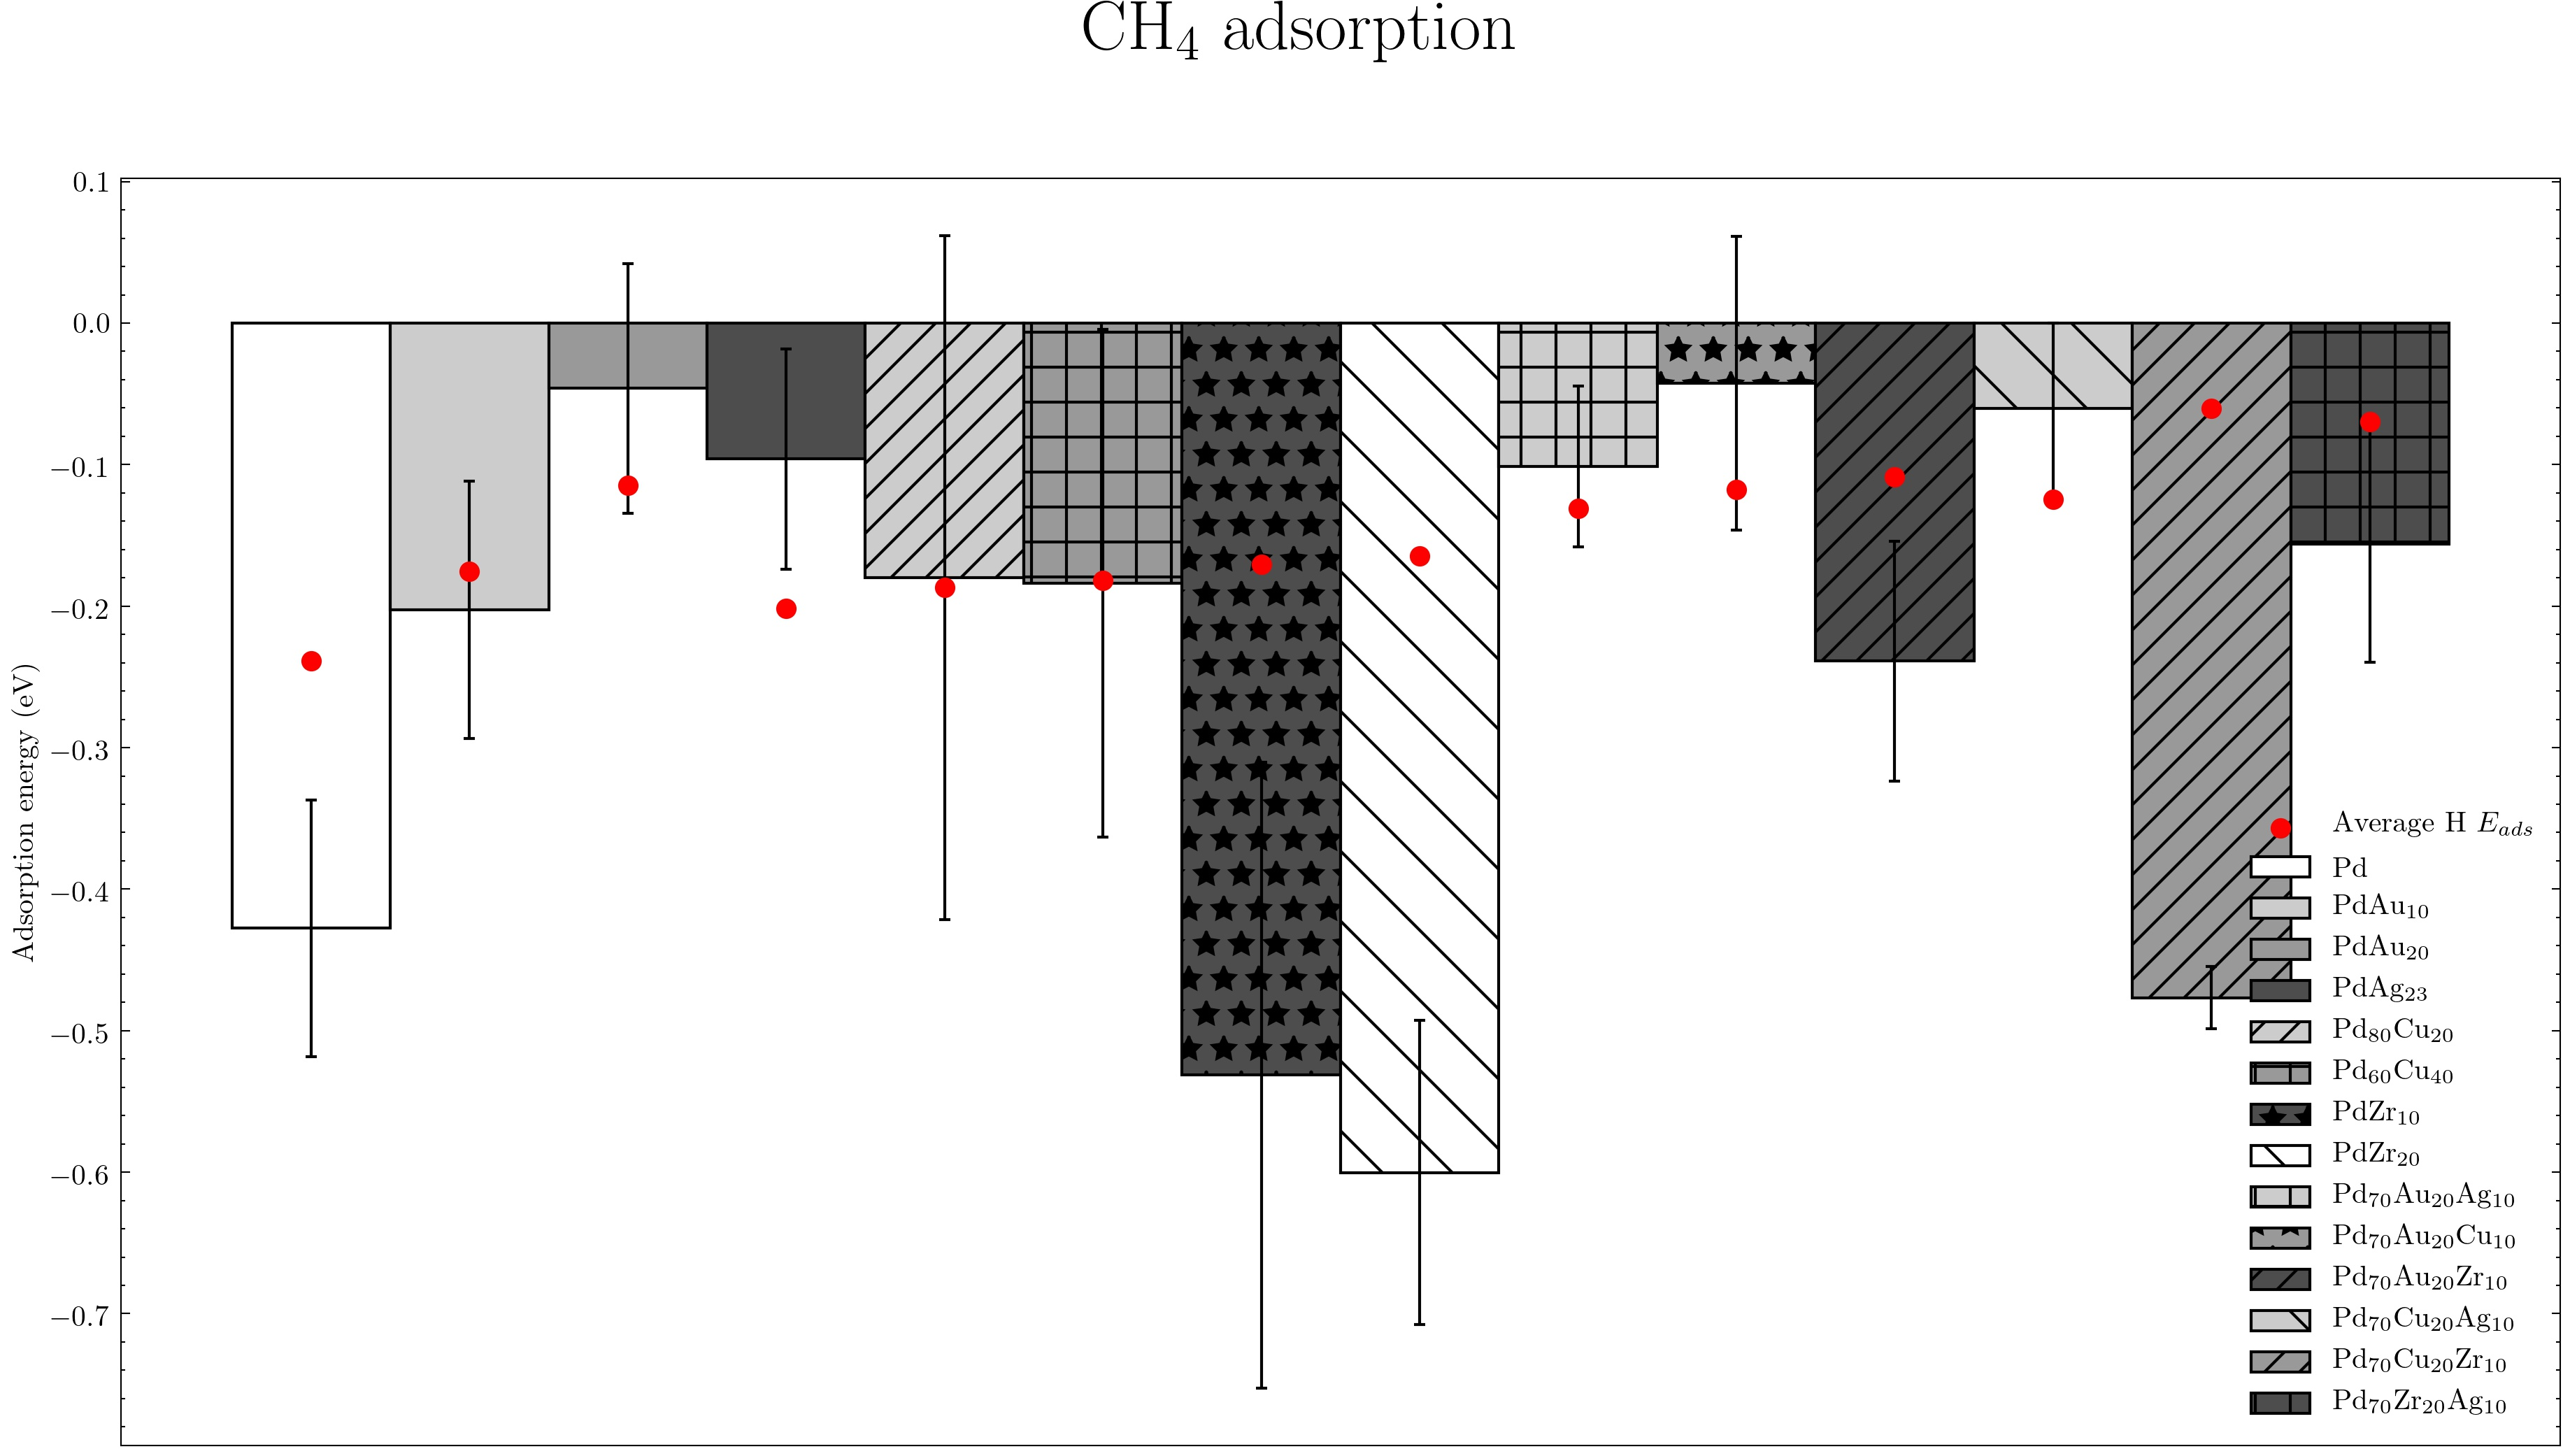
\includegraphics[width=0.9\linewidth,height=\textheight, keepaspectratio]{/Users/marc/Thesis/Chapter3/data/CH4ads.jpg}
      \caption{Average adsorption energy of Methane on the surface of palladium and palladium alloy slabs}
      \label{CH4ads}
    \end{figure}
  
  \end{landscape}
\subsubsection{Formaldehyde and Formic acid}
\begin{landscape}
  \begin{figure}
      \centering
      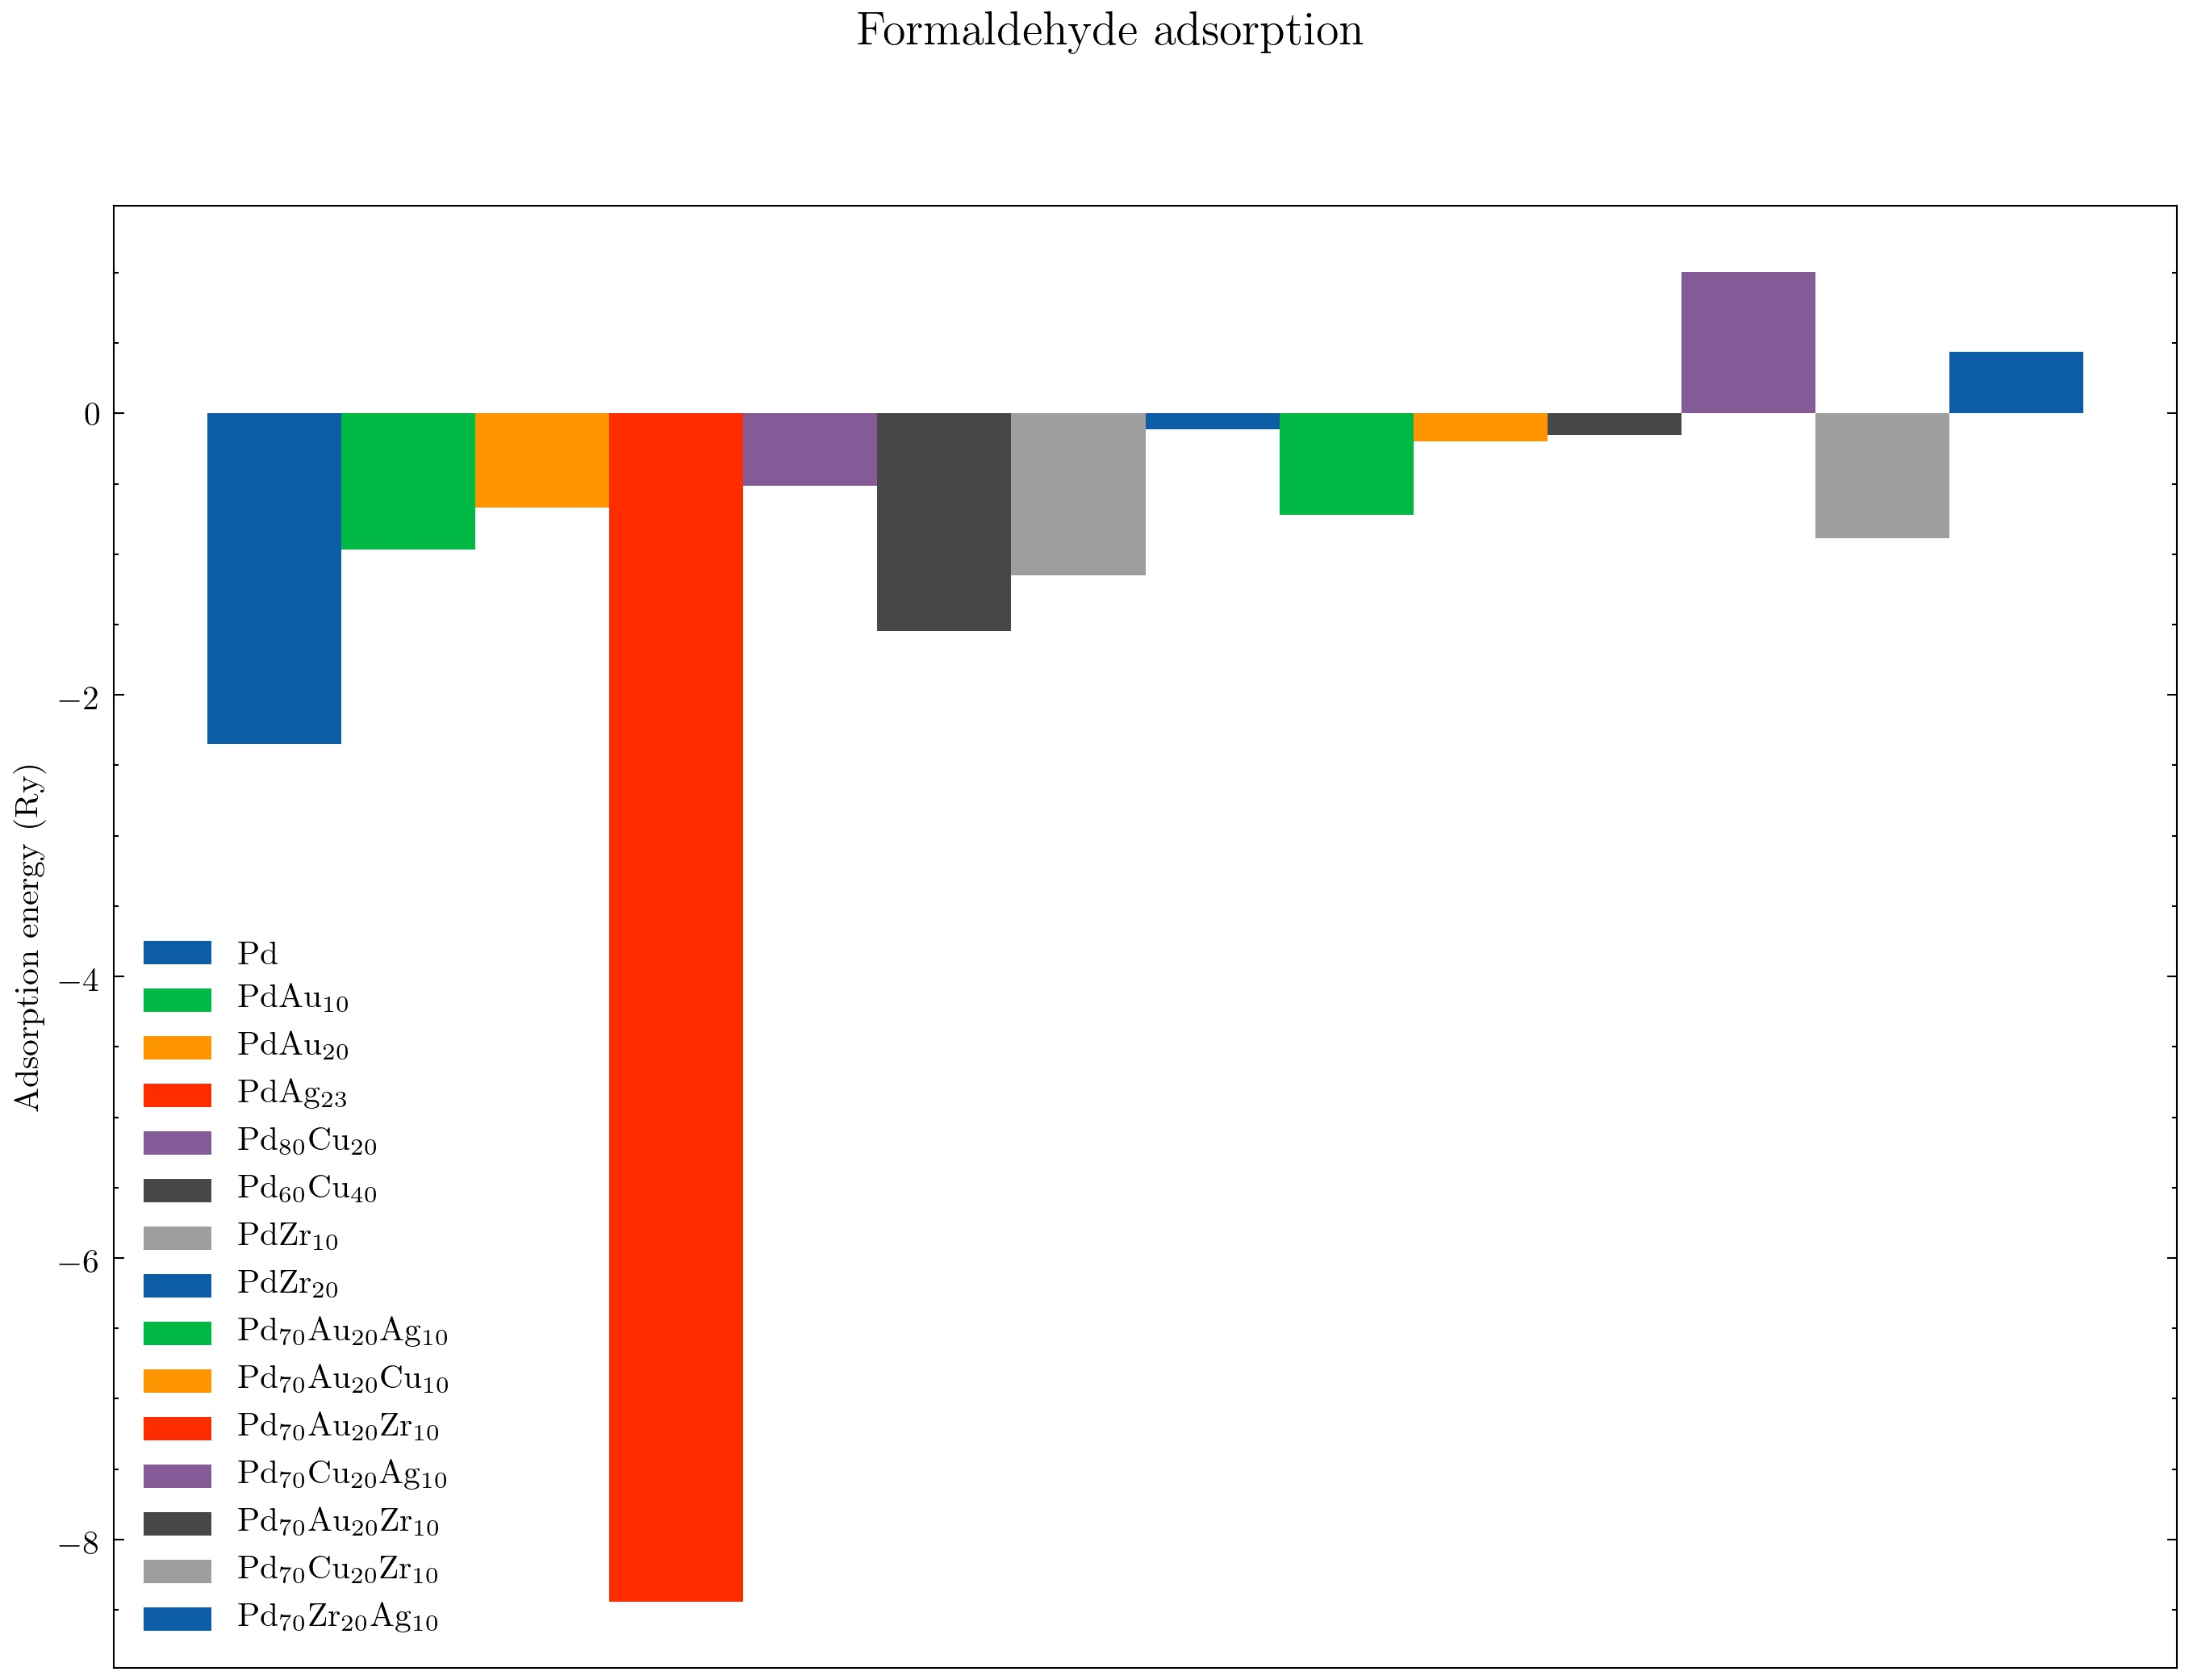
\includegraphics[width=0.9\linewidth,height=\textheight, keepaspectratio]{/Users/marc/Thesis/Chapter3/data/Formaldehydeads.jpg}
      \caption{Average adsorption energy of formaldehyde on the surface of palladium and palladium alloy slabs}
      \label{formaldehydeads}
    \end{figure}
  
  \end{landscape}

\begin{landscape}
  \begin{figure}
      \centering
      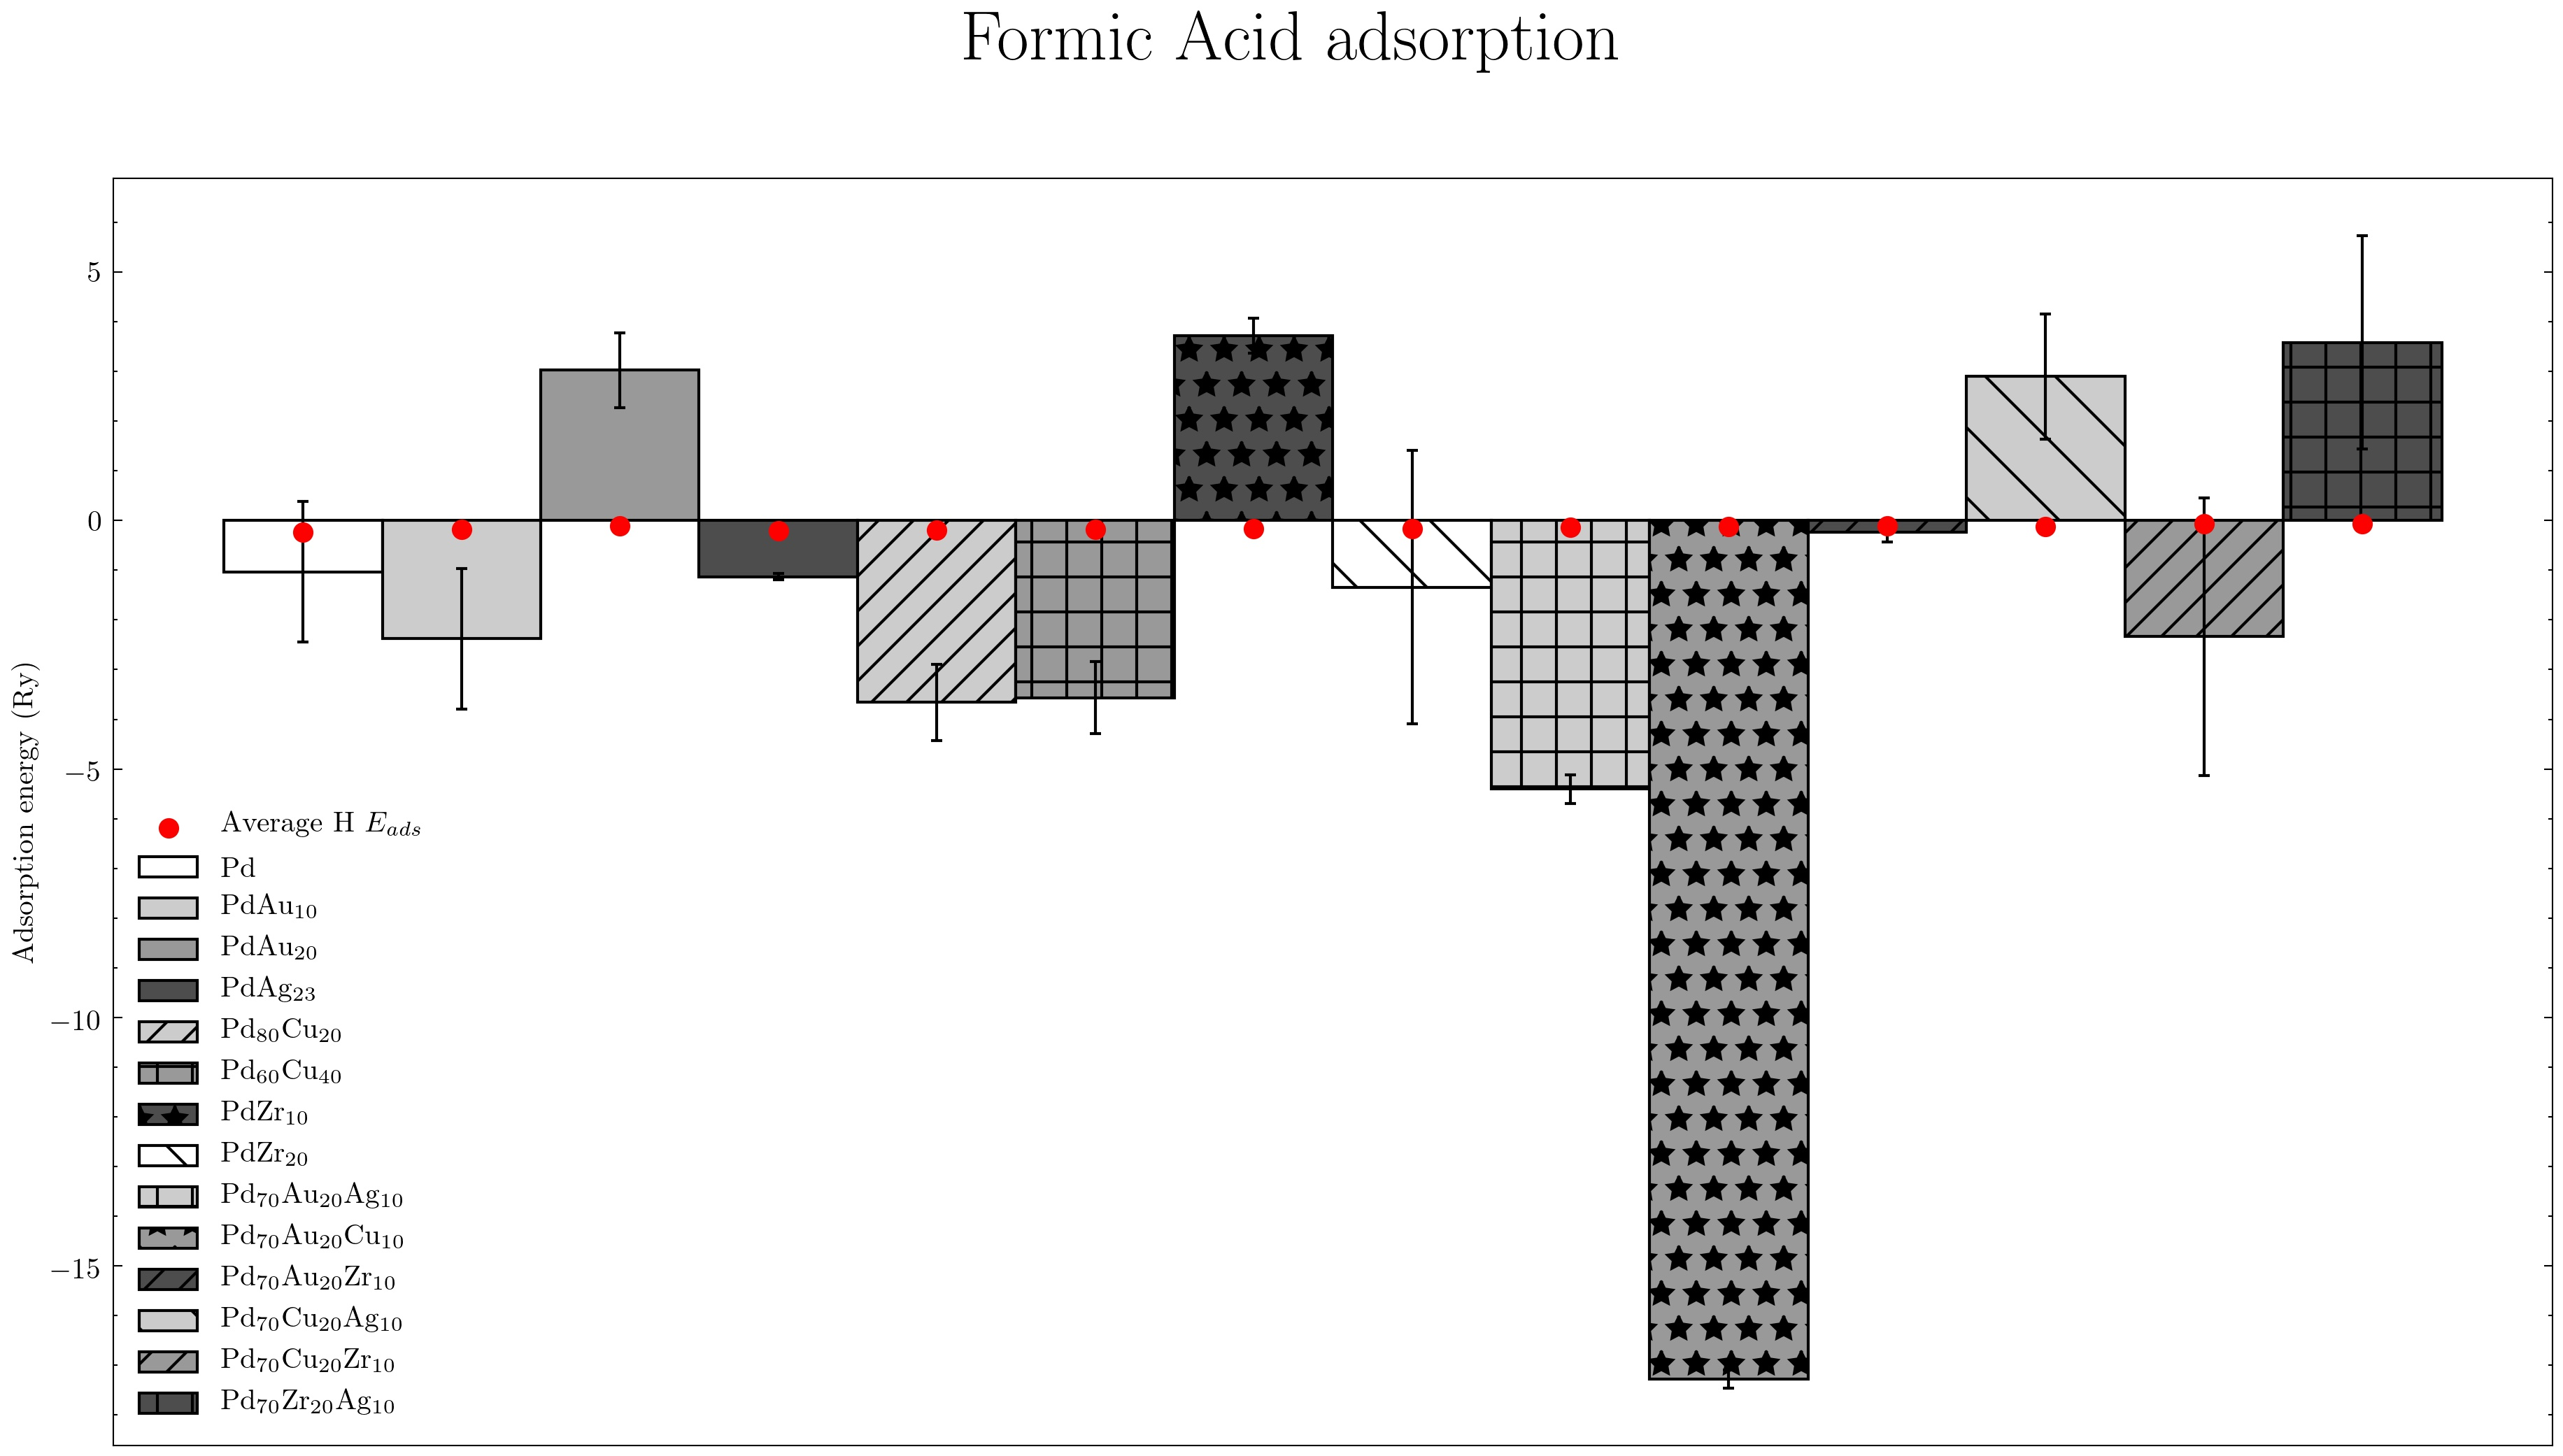
\includegraphics[width=0.9\linewidth,height=\textheight, keepaspectratio]{/Users/marc/Thesis/Chapter3/data/FAads.jpg}
      \caption{Average adsorption energy of Formic Acid on the surface of palladium and palladium alloy slabs}
      \label{FAads}
    \end{figure}
  
  \end{landscape}
\subsubsection{Hydrogen sulphide}
\begin{landscape}

\begin{figure}
    \centering
    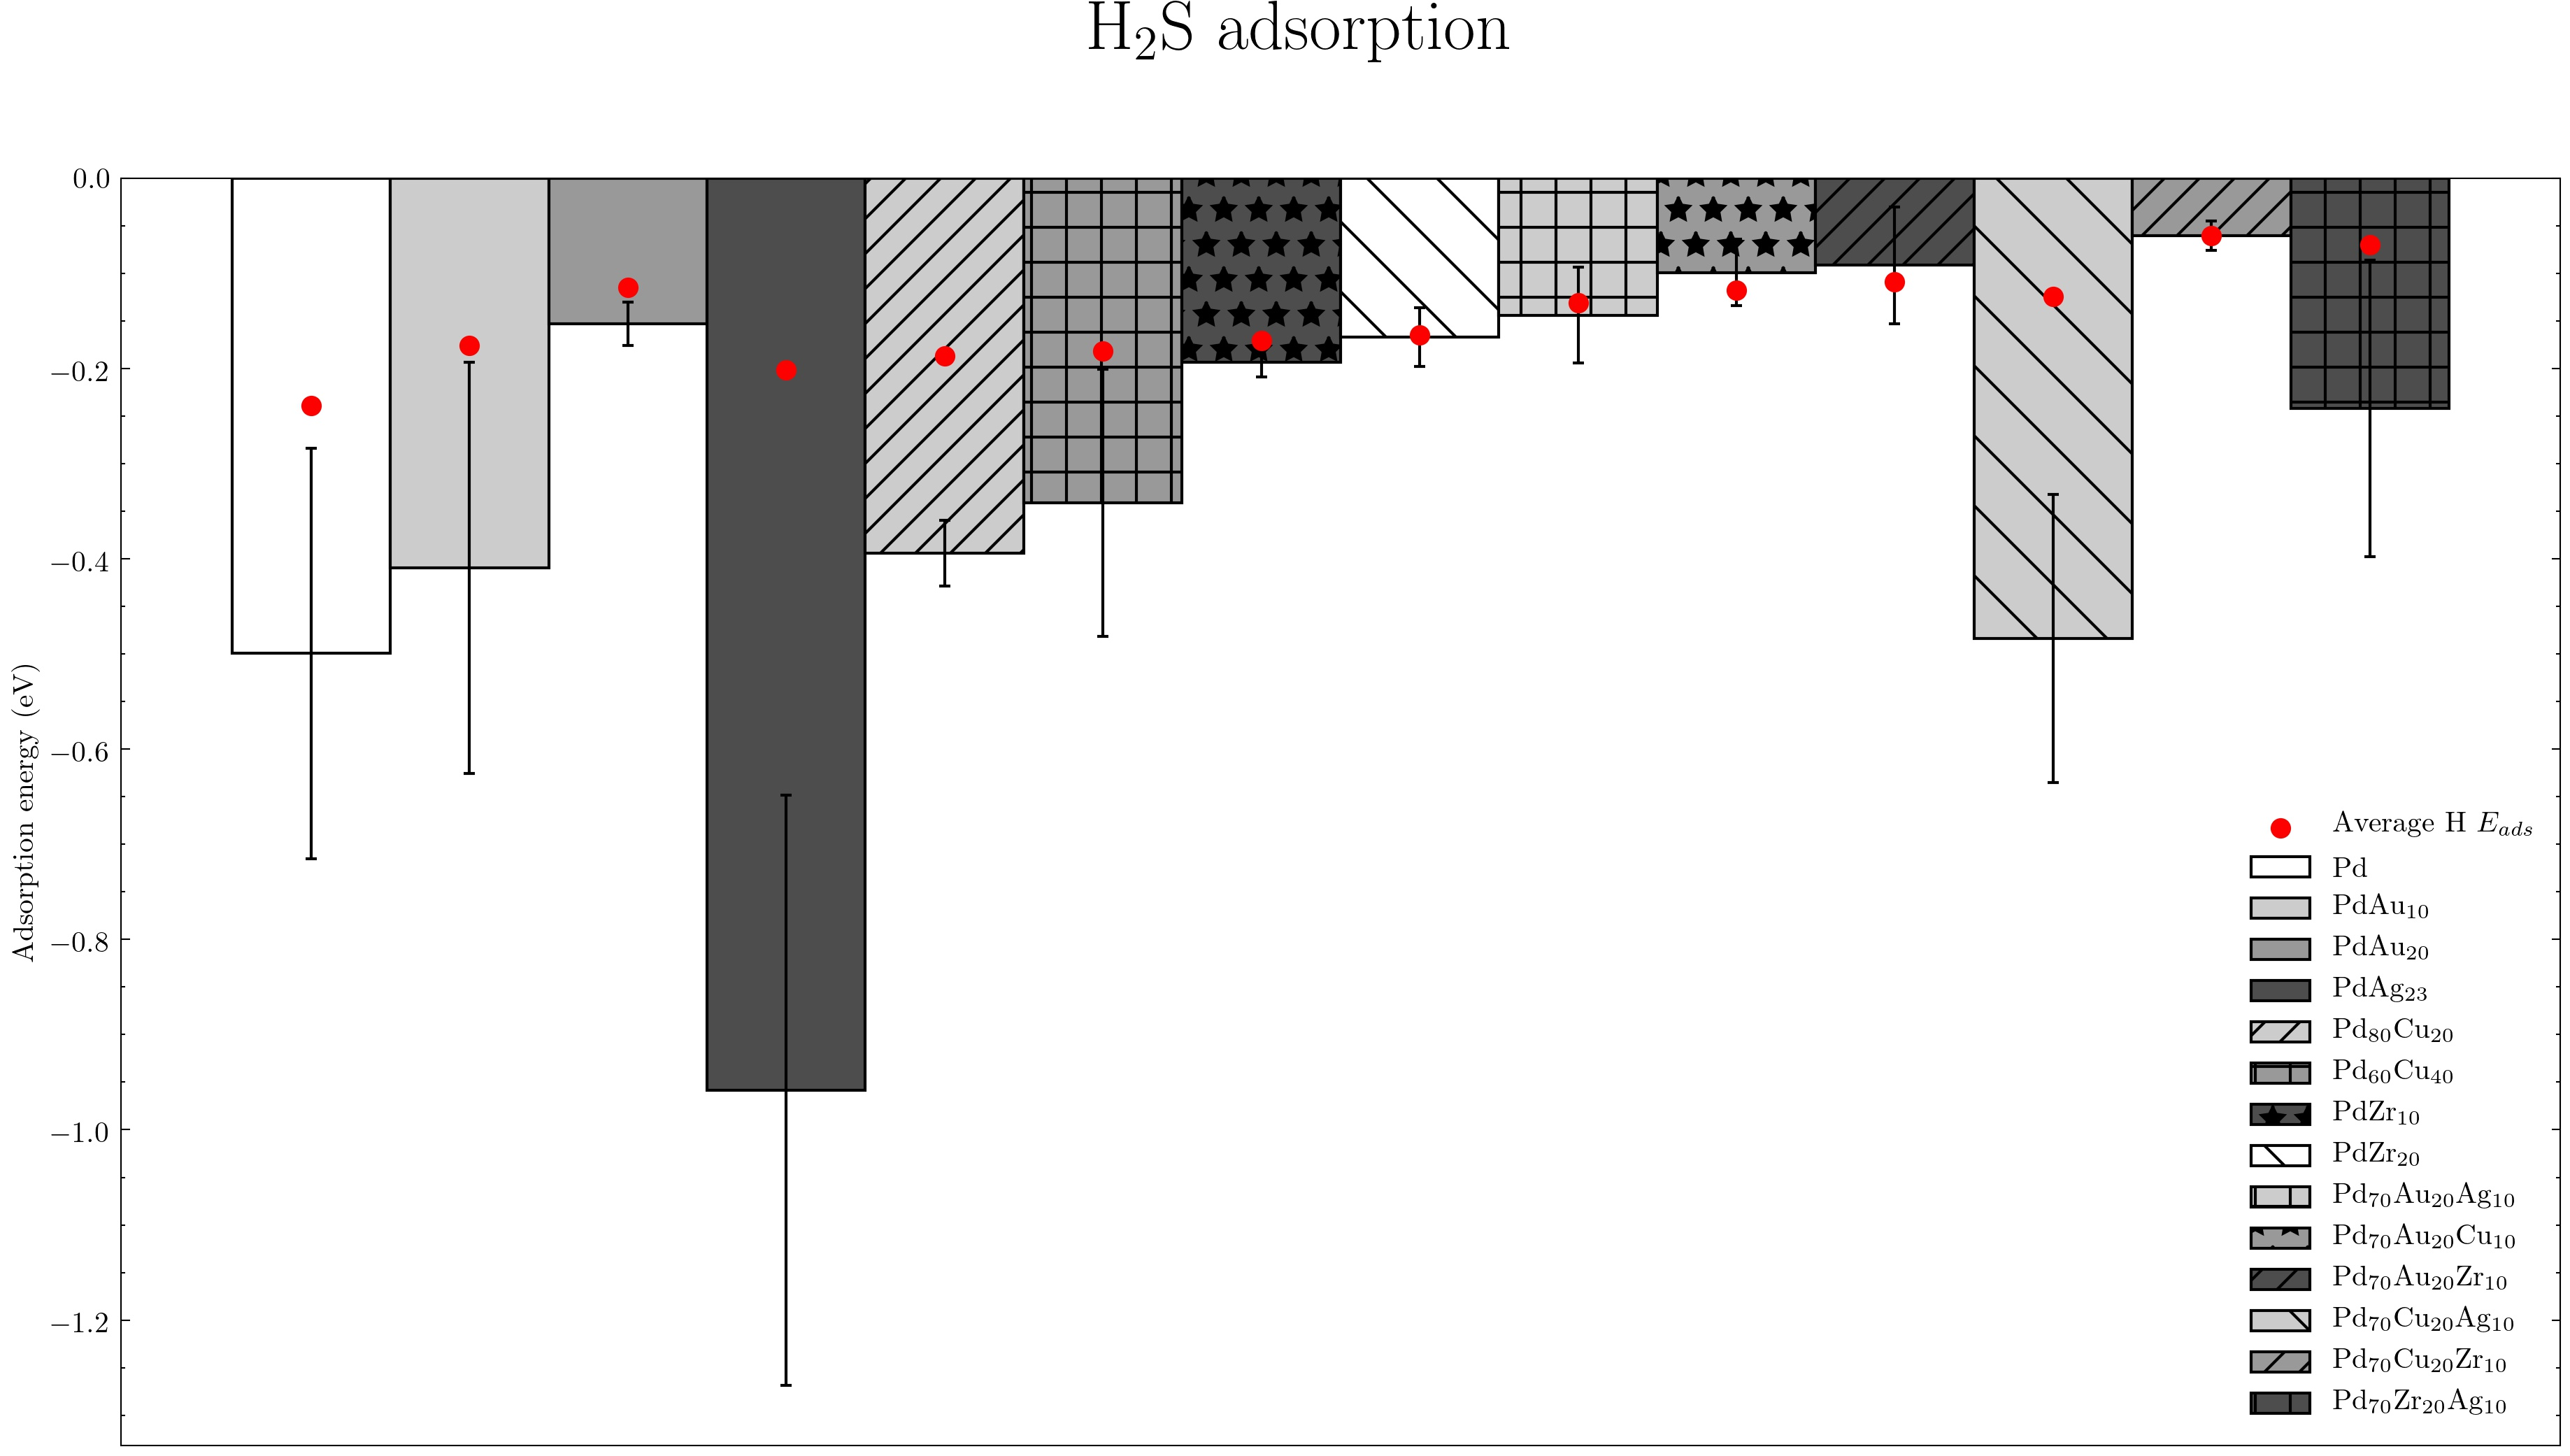
\includegraphics[width=0.9\linewidth,height=\textheight, keepaspectratio]{/Users/marc/Thesis/Chapter3/data/H2Sads.jpg}
    \caption{Average adsorption energy of H\textsubscript{2}S on the surface of palladium and palladium alloy slabs}
    \label{h2sads}
  \end{figure}
\end{landscape}


\section{Conclusion}
\bibliographystyle{unsrtnat}
\bibliography{library.bib}